\documentclass[a4paper, titlepage, openright]{book}

\usepackage[english]{babel}
\usepackage{frontespizio}
\usepackage{amsmath}
\usepackage{amsthm}
\usepackage[linesnumbered,ruled,vlined]{algorithm2e}
\usepackage{textcomp}
\usepackage{mathtools, nccmath}
\usepackage[left=3cm,right=2cm,top=3cm,bottom=2cm]{geometry}
\usepackage{rotating}
\usepackage{subfigure}
\usepackage{url}

% force page number on page bottom part
\usepackage{fancyhdr} 
\fancyhf{}
\cfoot{\thepage}
\pagestyle{fancy}

% These Commands create the label style for tables, figures and equations.
\usepackage[labelfont={footnotesize,bf} , textfont=footnotesize]{caption}
\captionsetup{labelformat=simple, labelsep=period}
\newcommand\num{\addtocounter{equation}{1}\tag{\theequation}}
\renewcommand{\theequation}{\arabic{equation}}
\makeatletter
\renewcommand\tagform@[1]{\maketag@@@ {\ignorespaces {\footnotesize{\textbf{Equation}}} #1.\unskip \@@italiccorr }}
\makeatother
\setlength{\intextsep}{10pt}
\setlength{\abovecaptionskip}{2pt}
\setlength{\belowcaptionskip}{-10pt}

\renewcommand{\textfraction}{0.10}
\renewcommand{\topfraction}{0.85}
\renewcommand{\bottomfraction}{0.85}
\renewcommand{\floatpagefraction}{0.90}

% This styles the bibliography and citations.
\usepackage{natbib}
\setlength\bibindent{2em}
\makeatletter
\setlength{\bibsep}{0pt plus 0.3ex}

% redefine chapter -> no labeling with 1, 2, etc.
\newcommand{\mychapter}[2]{
    \setcounter{chapter}{#1}
    \setcounter{section}{0}
    \chapter*{#2}
    \addcontentsline{toc}{chapter}{#2}
}

% table of contents will contain also subsections
\setcounter{tocdepth}{2}

% change Bibliography into References
\AtBeginDocument{\renewcommand{\bibname}{References}}

% set input and output for algorithm2e
\SetKwInput{KwInput}{Input}                
\SetKwInput{KwOutput}{Output} 

\begin{document}
% -----  title page
\begin{frontespizio}
	\Universita {Verona}
	\Dipartimento {Informatica}
	\Scuola {Ph.D. in Computer Science}
	\Annoaccademico {2021--2022}
	\Titoletto {Second Year Report}
	\Titolo {Predicting genetic variants effect on genome regulatory elements and CRISPR off-targets}
	\Candidato [VR456869]{Manuel Tognon}
	\NCandidato {Student}
	\NRelatore {Supervisor}{}
	\Relatore {Prof. Rosalba Giugno}
	\NCorrelatore {Cosupervisor}{}
	\Correlatore{Prof. Luca Pinello}
\end{frontespizio}
% ------  table of contents, index of figures and tables
\tableofcontents
\listoffigures
\listoftables
% ------ Introduction
\mychapter{1}{Introduction}
% ------ Transcription Factors
\mychapter{2}{Transcription Factors}
Transcription Factors (TFs) (\textbf{Fig.\ref{fig:ctcf_dna}}) are fundamental regulatory proteins playing a key role in regulating the transcriptional state, differentation and developmental state of cells \citep{lambert2018human, reimold2001plasma, whyte2013master}. TFs present a modular structure, divide in three domains \citep{latchman1997transcription}: (i) the DNA binding domain, (ii) the activation domain, and (iii) the signal sensing domain. The DNA binding domain guides the TF to the its target sites on the genome. The activation domain interacts with other transcriptional reagulators. The signal sensing domain captures external signals, transmitting them to the whole transcriptional complex. In human, about 1600 proteins are currently thought to function as TFs \citep{babu2004structure}. Therefore, approximately the $8$\% of human genes encode for TFs. Transcription Factors often exploit their regulatory function on genes, by acting in a coordinate fashion. Moreover, TFs regulate multiple genes in different cell-types \citep{lambert2018human}. TFs perform their regulatory function by employing different strategies: (i) helping or blocking RNA polymerase binding \citep{fuda2009defining}, (ii) weakining the DNA-histones associations opening the chromatin, (iii) catalyzing histones deacetylation \citep{liu2016beyond}, or (iv) strengthening the DNA-histone complexes closing the chromatin. By binding short DNA sequences (7-20 nucleotides \citep{stewart2012transcription}) called Transcription Factor binding sites (TFBS), TFs finely regulate gene expression in a cell-specific manner. TFBS are located within gene promoters \citep{whitfield2012functional} or in distal regulatory elements, such as enhancers, silencers or insulators \citep{gotea2010homotypic,lemon2000orchestrated,nolis2009transcription}. Although TFBS show recurring sequence patterns, which are often are referred to as \emph{motifs}, TFs bind similar but not identical sequences, that can differ in a few nucleotides. The precise identity and configuration of TFBS, together with the conformation of flanking chromatin regions, critically regulate TFs regulatory function of cells \citep{mendenhall2013locus,maurano2015large}. During DNA binding, Transcritpion Factors use a combination of electrostatic and Van der Waals forces. Although TFs bind their target sequences with high specificity, not all nucleotides in the binding sites directly interact with the TF. Since some interactions between the TF and the TFBS nucleotides are weaker than others, TFs do not bind a single signal sequence, but a subset of a closely related targets. However, the sequence composition defines the TF-DNA binding strength (binding affinity). Several studies linked different diseases and cancer types to gentic variants occurring in TFBS \citep{docquier2005heightened, katainen2015ctcf, yu2019gata1}. Moreover, the misregulation of gene expression governed by TFs caused by variants occurring in TFBS could affect the entire cell environment and be propagated to neighboring cells. Therefore, identifying such regulatory motifs would provide fundamental insights on the complex mechanisms governing gene expression and the cell environment.
\begin{figure}
	\centering
	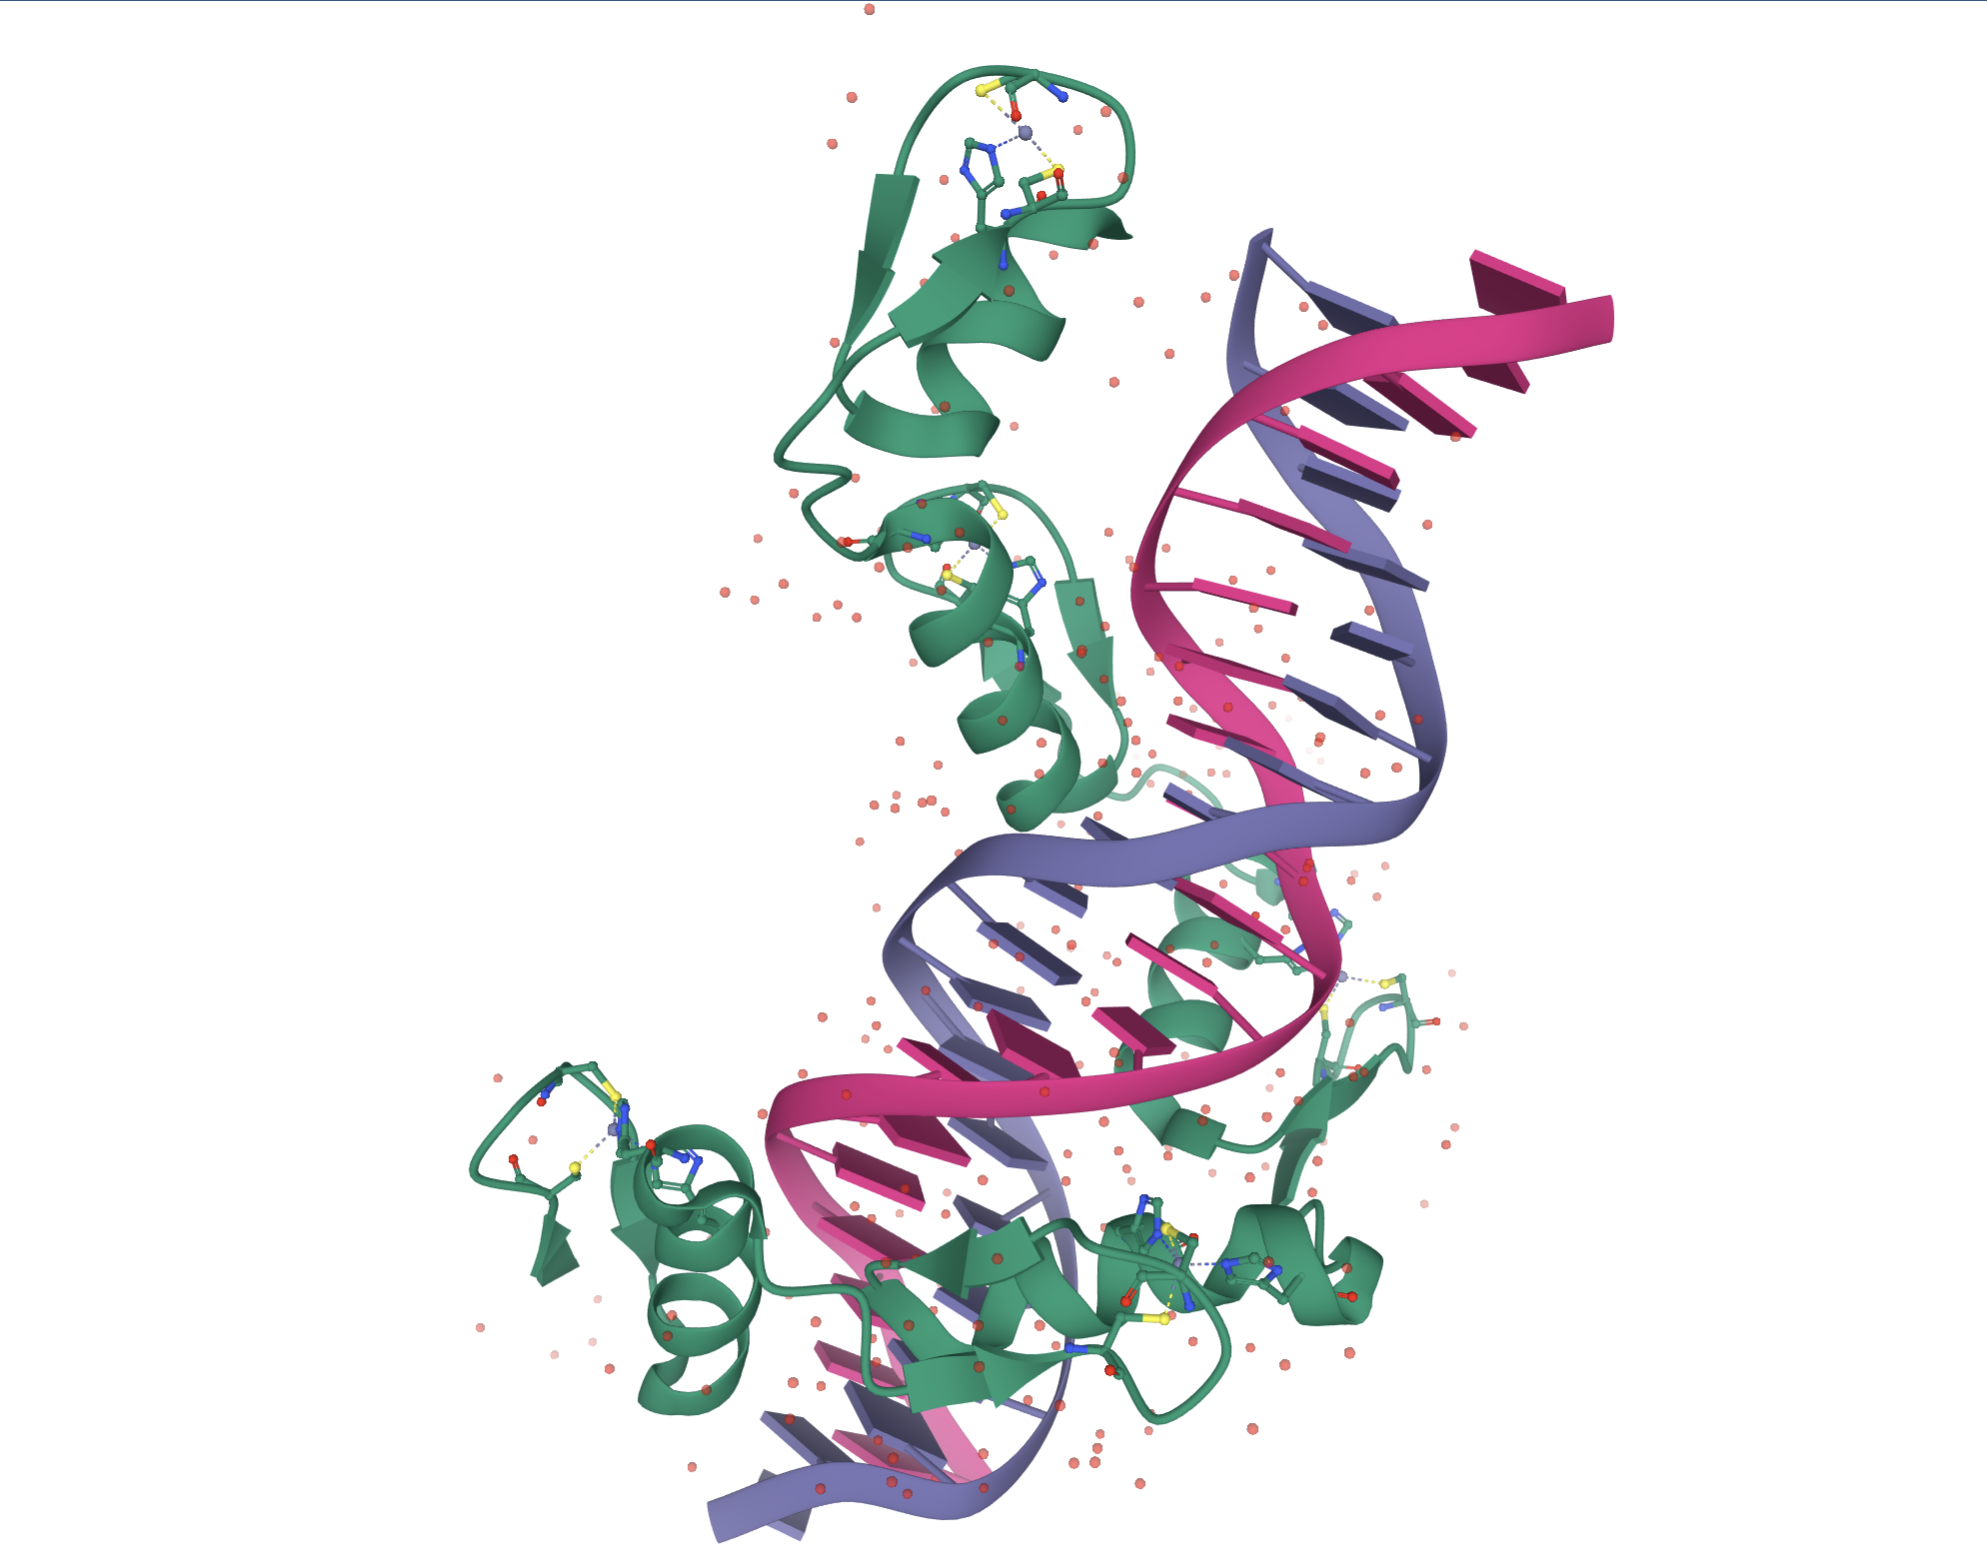
\includegraphics[width=\textwidth]{figures/ctcf_dna.png}
	\caption[A human transcription factor (CTCF) binding its DNA target sequence.]{\textbf{A human transcription factor (CTCF) binding its DNA target sequence.}}
	\label{fig:ctcf_dna}
\end{figure}
% ---- Discovering Transcription Factor Binding Site motifs
\section{Discovering Transcription Factor Binding Site motifs}
Several experimental assays have been developed to determine the binding site sequences of TFs in living cells or organisms (\emph{in vivo}), or in test-tubes using synthetic or purified components (\emph{in vitro}) \citep{jolma2011methods}. Early methods, like electrophoretic mobility shift assay (EMSA) \citep{garner1981gel} or footprinting \citep{hampshire2007footprinting}, generally search the binding sites for the investigated TFs analyzing a relatively small number of target sequences, producing small datasets of bound sequences. The introduction of in vitro and in vivo high-throughput protocols, like PBM, SELEX or ChIP methods \citep{berger2006compact,jolma2010multiplexed,collas2008chop}, enabled the analysis of most of all possible target sites for the investigated factors, returning large datasets of bound sequences, and providing an unprecedented opportunity to study and determine TFs binding landscapes. Experimental assays can recover the bound sequences along with their binding affinity values. However, such datasets can hide unbound sequences erroneously reported as binding sites (false positives). Moreover, most assays capture several additional nucleotides the target sites, limiting the data resolution, and making manual analyses difficult and often unfeasible. Motif discovery algorithms provide a computational framework to analyze the datasets produced by experimental assays, discovering the sequences potentially bound by TFs and reporting their predicted affinities. Given a sequence dataset, motif discovery algorithms recover sets of short and similar sequence elements. The prioritized sequence elements are later used to construct a motif model, summarizing the diverse binding site configurations observed among the prioritized sequences, and encoding their recurrent patterns and similarities. The development of motif discovery methods is one of the most investigated and active research fields in computational biology \citep{pavesi2004silico,tompa2005assessing,d2006does,das2007survey,zambelli2013motif}. Several different algorithms and models have been proposed to discover and represent TFBS motifs. Position weight matrices (PWMs) \citep{stormo2000dna} are the most popular models to represent TFBS motifs. PWMs are powerful and interpretable models, encoding the probability of observing a given nucleotide in each TFBS position. However, PWMs have some limitations, like the assumption of independence among the binding site positions. Therefore, several alternative models have been proposed to describe TFBS motifs \citep{siddharthan2010dinucleotide,gorkin2012integration,he2021survey}. The derived motif models can be employed in many downstream analyses, like searching potential binding site occurrences in regulatory genomic sequences, predicting the sets of genes regulated by the investigated TFs, or assessing how genetic variants could affect the factors’ binding landscape.
% -- Experimental methods to discover Transcription Factor Binding Sites
\begin{table}
	\centering
	\begin{tabular}{|p{2.4cm}|p{4cm}|p{1.75cm}|p{1.5cm}|p{1cm}|p{2.3cm}|p{2cm}|}
		\hline
		\textbf{Experimental assay}& \textbf{Description}&\textbf{Output}&\textbf{\emph{De novo} motif discovery capability}& \textbf{Type}& \textbf{Identification of genomic binding locations}& \textbf{Throughput} \\
		\hline
		Competition EMSA& Bound DNA sequences are identified by observing changes in the electrophoretic migration of DNA sequences through non-denatured polyacrylamide gel.& Bound DNA sequences.& No. Used to validate known binding sites.& \emph{in vitro}& No& Low\\  
		\hline
		DNase footprinting& Pools of DNA sequences are incubated with the TF of interest; then, the DNA is degraded using DNase-I. The unbound fragments are cut in all positions, while the bound DNA is protected by the TF.& Bound DNA sequences.& No. Used to validate known binding sites.& \emph{in vitro}& No& Low\\
		\hline
		Protein Binding Microarrays& Arrays of ~40,000 spots with short immobilized DNA sequences are incubated with a  GST-tagged TF, and then washed to remove weakly bound proteins. The bound sequences are identified through fluorescence-based detection.& Continuous values describing fluorescence intensity on each array spot.& Yes. Limited to short motifs (~12bp).& \emph{in vitro}& No& High\\
		\hline
		HT-SELEX& The TF is added to a pool of randomized DNA fragments. The bound sequences are selected and constitute the starting pool for the next experimental round. The procedure is repeated for several rounds. Sequencing is employed to recover the sequence of the bound DNA fragments.& DNA sequences.& Yes& \emph{in vitro}& No& High\\
		\hline
		ChIP-based technologies& TF-DNA complexes are crosslinked with formaldehyde, and immunoprecipitated employing TF-specific antibodies. The bound sequences are then prioritized employing qPCR microarrays (ChIP on Chip) or through sequencing (ChIP-seq). ChIP-exo integrates exonuclease treatment to enhance sequence resolution.& Genomic binding location coordinates.& Yes. Limited by the inability to distinguish direct and indirect binding.& \emph{in vivo}& Yes& Low\\
		\hline
	\end{tabular}
	\caption[In vivo and in vitro experimental assays to identify and validate Transcription Factor binding sites.]{\textbf{In vivo and in vitro experimental assays to identify and validate Transcription Factor binding sites.} Generally, EMSA and DNase footprinting are used to validate known TFBS, while currently PBMs, HT-SELEX, and ChIP-based methods are preferred to discover novel binding sites. Importanlty, ChIP-based assays are the only methods that recover the TF genomic binding locations. The throughput column refers to the number of samples that can be processed in parallel by each method (high: about hundreds of samples; low: few samples).}
	\label{table:assays}
\end{table}
\begin{figure}
	\centering
	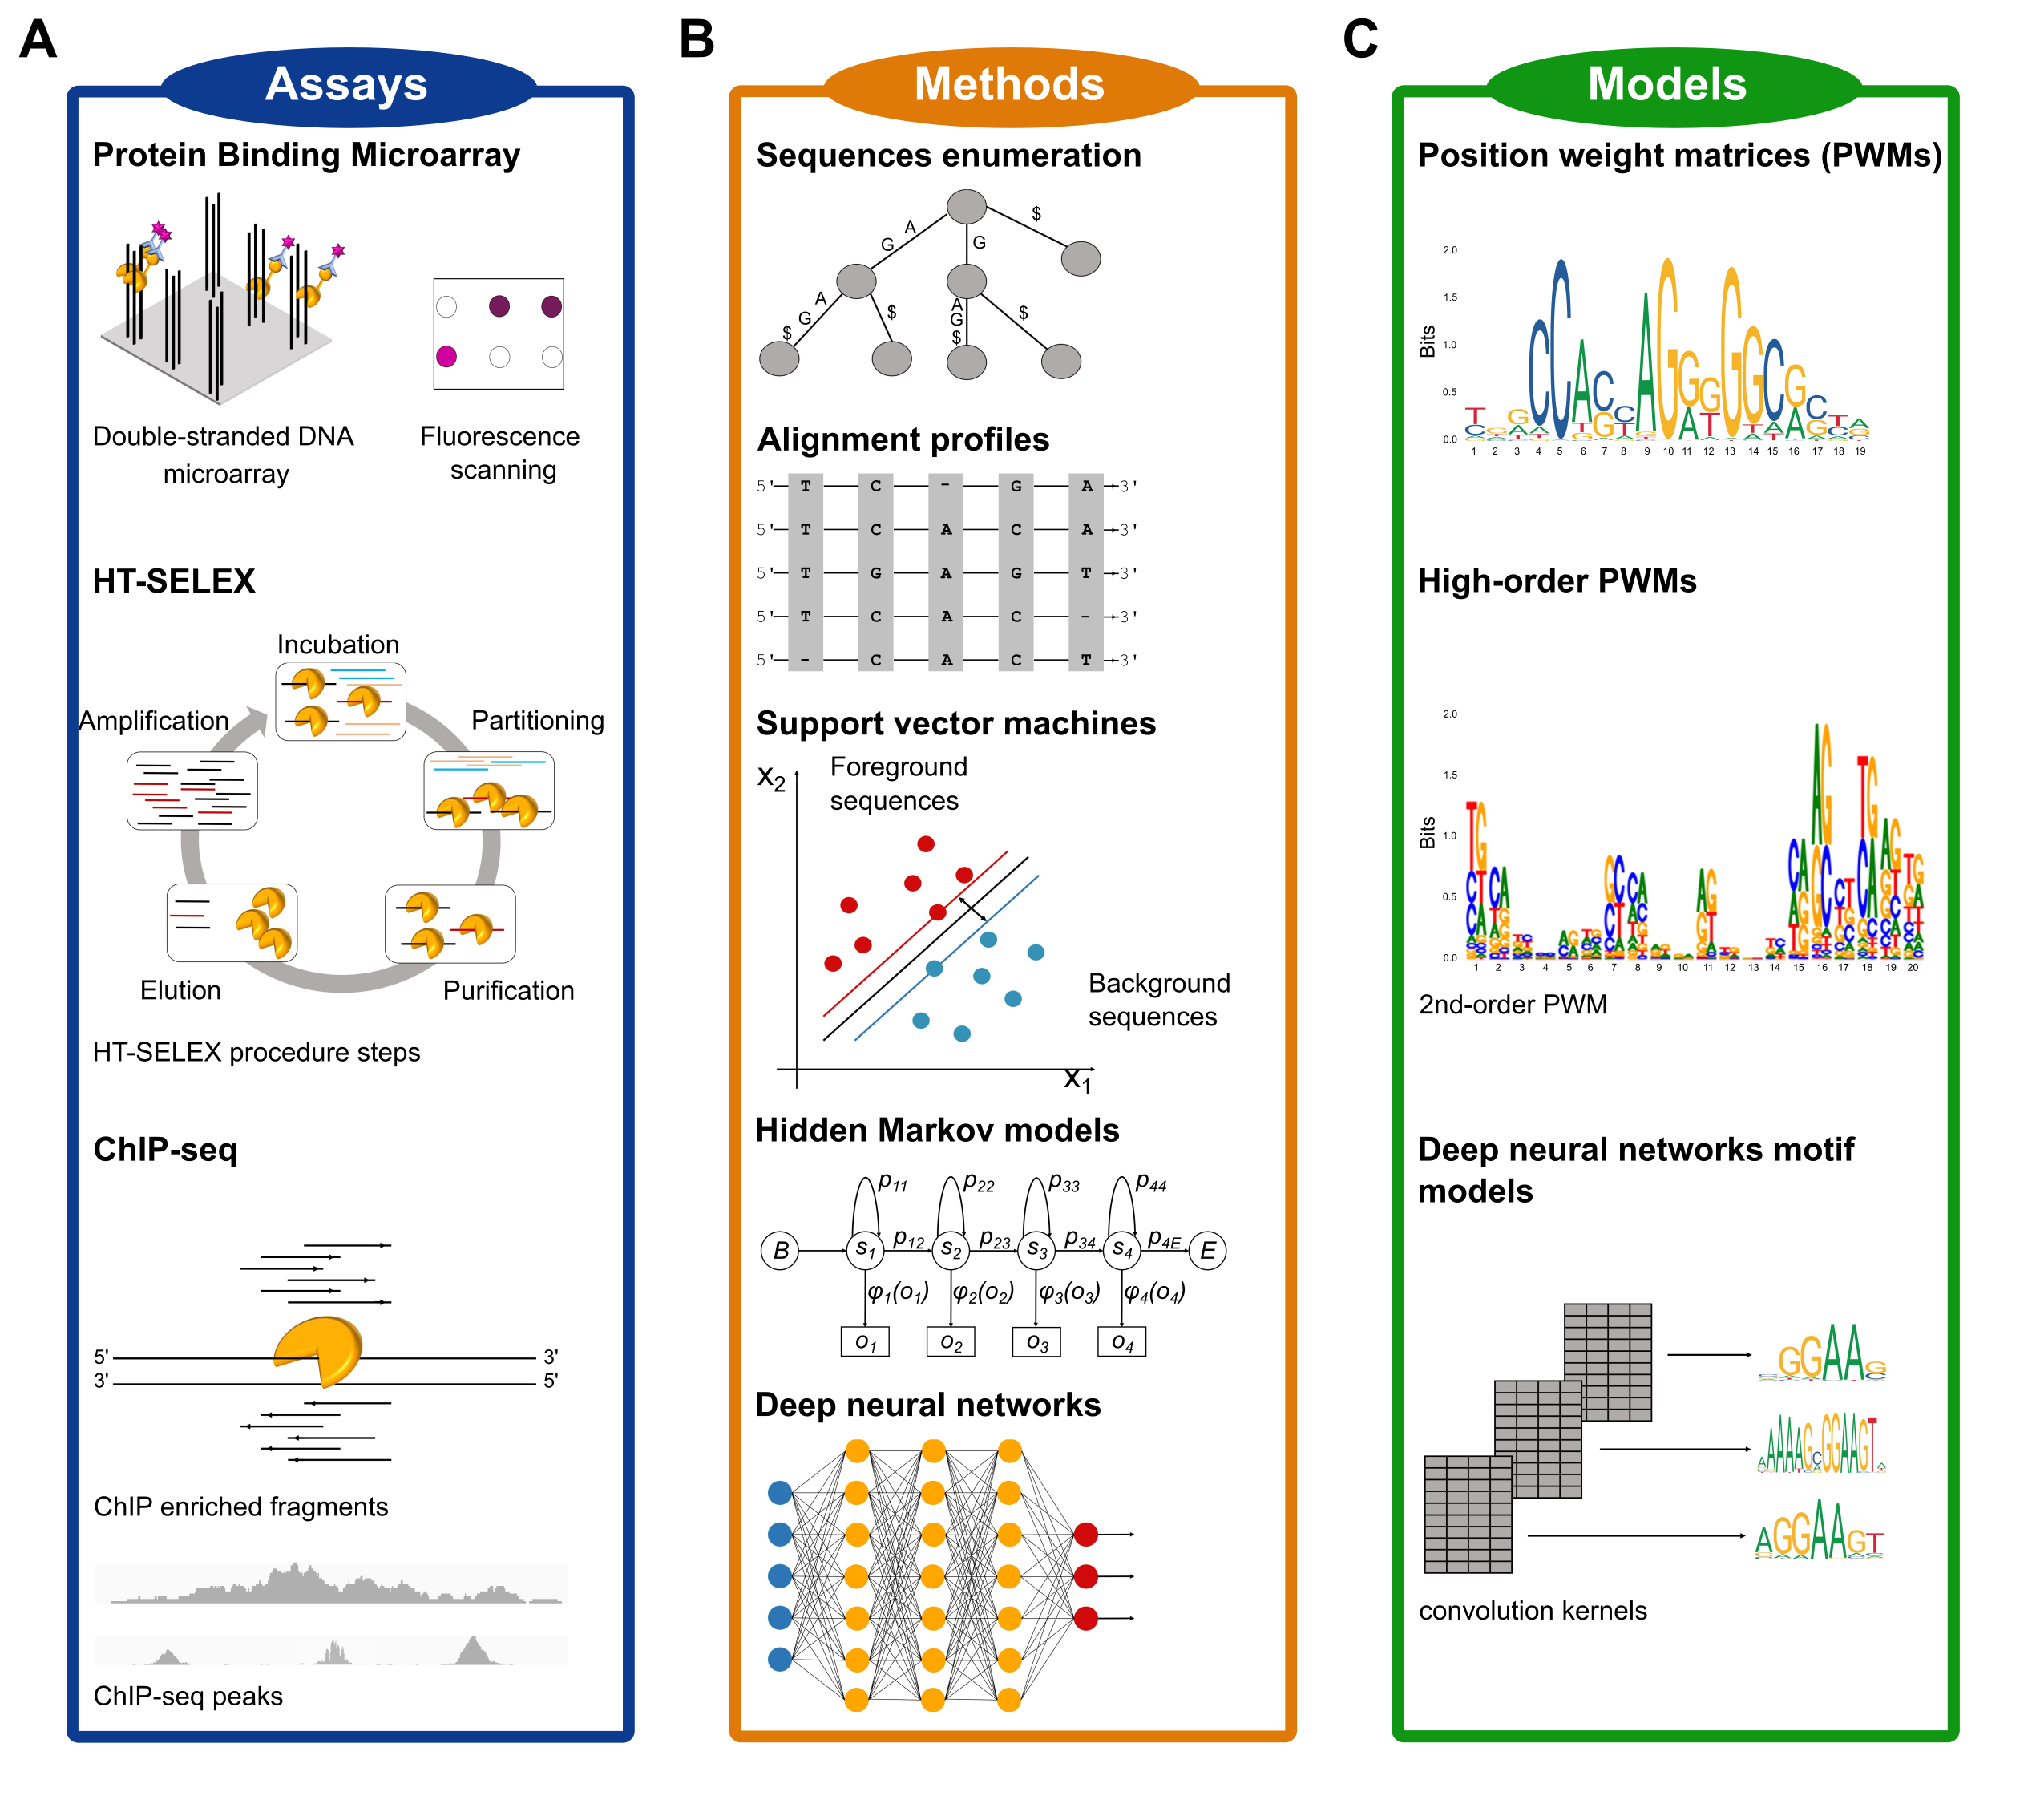
\includegraphics[width=\textwidth]{figures/md.png}
	\caption[Experimental and computational methods to discover TFBS and popular models to represent binding site motifs.]{\textbf{Experimental and computational methods to discover TFBS and popular models to represent binding site motifs. (A)} Protein binding microarray (PBM), HT-SELEX and ChIP-seq during the last years have become the most popular assays to determine TF binding profiles and identify their target sites (TFBS). \textbf{(B)} Computational motif discovery methods can be grouped in five classes, based on the algorithms employed to discover TFBS: enumerative, alignment-based, probabilistic graphical models-based, support vector machines (SVMs), and deep neural network (DNN) based methods. \textbf{(C)} TFBS sequences prioritized by motif discovery algorithms are encoded in computational models representing the binding preferences of the investigated TFs. }
	\label{fig:md}
\end{figure}
\subsection{Experimental methods to discover Transcription Factor Binding Sites}
During the last decades, several techniques have been introduced to experimentally identify and assess TF binding sites and binding preferences \citep{jolma2011methods} (\textbf{Fig.\ref{fig:md} (A)} and \textbf{Table \ref{table:assays}}). Early studies on TF binding focused their analysis on gene promoters \citep{stormo2000dna} and employed in vitro methods, such as Electro-Mobility Shift Assay (EMSA) \citep{garner1981gel} or DNase footprinting \citep{galas1978dnaase}. EMSA exploits non-denatured polyacrylamide gel properties to separate bound and unbound DNA sequences, while DNase footprinting combines EMSA with DNase I cleavage. Generally, these assays produce datasets of a few hundreds of bound sequences, exploring a limited spectrum of TFs binding landscape. Moreover, EMSA and DNase footprinting often suffer from high false positive rates due to the identification of unwanted protein-DNA interactions, caused by nonspecific DNA binding factors potentially leading to wrongly measured binding preferences \citep{jolma2011methods}. The introduction of NGS technologies revolutionized the study of TFBS identification by encouraging researchers to develop methods that exploit the power of massively parallel sequencing, to identify TFBS. These methods have two major advantages: (i) they do not require any prior knowledge on the binding site sequence \citep{jolma2011methods,zia2012towards}, and (ii) produce datasets of thousands of bound sequences allowing to better characterize TFs binding preferences \citep{stormo2010determining}. Protein binding microarrays (PBMs) \citep{berger2006compact,berger2009universal} recover short TFBS sequences (~10 bp), and measure TF binding preferences in vitro. In PBMs a tagged TF is released on a glass slide containing thousands of spots filled with short immobilized DNA sequences. The tagged TFs are then incubated with fluorescent antibodies against the tag and subsequently washed to remove weakly bound factors. The fluorescence and DNA sequence enrichment are then used to quantify the TF-DNA binding strength and capture the bound sequences. Generally, the recovered sequences do not contain nucleotides flanking the investigated binding sites, producing high resolution datasets. However, since the number of possible sequences grows as a function of the target length, PBMs can assess only a limited number of target sequences \citep{jolma2011methods,zia2012towards}. Therefore, PBMs analysis is usually constrained to binding sites ~10-12 bp long.  HT-SELEX \citep{jolma2011methods,jolma2010multiplexed} is a widely used in vitro method, coupling SELEX with high throughput sequencing. A TF is released on a pool of randomized DNA sequences, to allow the factor to select its target sites. The resulting TF-DNA complexes are separated from unbound sequences, and subsequently amplified through PCR and sequenced. The resulting DNA library is enriched in binding sites for the studied TF and is used as the starting pool for another SELEX run \citep{jolma2011methods,jolma2010multiplexed}. SELEX captures the binding preferences of TFs without requiring any prior knowledge on their target sites \citep{collas2008chop}. Since SELEX reaction is typically performed in liquid phase and consequently does not suffer from physical constraints, the sequence space covered by HT-SELEX is often larger than that of PBMs. Moreover, by coupling sequencing with DNA barcode indexing, HT-SELEX allows to analyze of hundreds of TFs in a single run. HT-SELEX produces datasets of thousands of high resolution bound sequences, which include only a few nucleotides flanking the binding sites. However, since the starting DNA library is constituted by randomized sequences, HT-SELEX cannot recover the genomic binding locations for the investigated factor. The introduction of chromatin immunoprecipitation (ChIP) technologies \citep{collas2008chop} radically changed the study of TFBS binding, enabling the genome-wide identification of regions bound by TFs in vivo. In ChIP the TF-DNA complexes are cross-linked using formaldehyde. The DNA is then fragmented in ~100-1000 bp long fragments, and subsequently immunoprecipitated with antibodies specific for the investigated TF. To recover the bound sequences, the cross-links are reverted. Then, the resulting fragments are amplified through microarray hybridization (ChIP on Chip \citep{collas2008chop,pillai2015chip}), or sequencing (ChIP-seq \citep{johnson2007genome,mardis2007chip}). To locate the binding regions, the recovered DNA fragments are mapped onto the genome. After ChIP-seq reads mapping, peak calling algorithms \citep{thomas2017features,guo2012high,zhang2008model} are employed to predict the genomic binding locations for the investigated factor. Peak calling algorithms identify the genomic regions showing greater enrichment in mapped DNA probes with respect to a control experiment (ChIP-seq peaks), and mark those regions as binding locations, or peaks \citep{pepke2009computation}. ChIP methods produce large datasets of thousands of genomic regions enriched in TFBS, whose length ranges from few hundreds to thousands of nucleotides. Although ChIP technologies, and particularly ChIP-seq, are currently considered the current 'golden standard', they have several limitations. (i) experimental results are influenced by chromatin states (most TFs bind only open chromatin [1]). (ii) ChIP can detect indirect binding, identifying other TFBS not belonging to the investigated factor \citep{worsley2014non}. (iii) ChIP-seq peaks may be false positives, recovered because of poor antibody quality, for example \citep{pickrell2011false}. (iv) ChIP-seq returns low resolution datasets, whose sequences include several nucleotides flanking the target TFBS. ChIP-exo \citep{rhee2011comprehensive} addresses the latter issue, employing a lambda exonuclease to trim ChIP sequences, removing some of the nucleotides flanking the target sites. In summary, the current high-throughput assays produce large datasets consisting of thousands of sequences potentially containing all possible binding configurations of TFBS allowing a better characterization of TFs binding landscapes. However, the sequences recovered by most of the described methods contain nucleotides flanking the TFBS, and only PBMs and HT-SELEX data marginally suffer marginally from this issue. Therefore, computational methods and models to identify and characterize TFBS become fundamental to exploit the information contained in the datasets produced by experimental assays.
% -- Computational methods to discover Transcription Factor Binding Sites
\subsection{Computational methods to discover Transcription Factor Binding Sites}
TFBS motif discovery is one of the most investigated problems in computational biology \citep{tognon2022survey}. During the last decades, several different algorithmic approaches have been proposed to discover potential binding sites in DNA sequences: \emph{enumerative}, \emph{alignment-based}, \emph{probabilistic graphical models}, \emph{support vector machines-based}, and \emph{deep neural network-based} methods (\textbf{Fig.\ref{fig:md} (B)}). Regardless of the algorithms employed and the computational model used to represent TFBS motifs, the TFBS motif discovery problem can be formalized as follows. Given a set of positive DNA sequences $S$, obtained from an experimental assay targeting a certain TF, and a set of negative sequences $B$, the goal is to find one or more recurrent, short and similar subsequences in $S$, that maximize the discriminatory power between $S$ and $B$. Such subsequences are called patterns or motifs, and are likely bound by the investigated TF. The negative set $B$ can contain randomly generated or selected genomic sequences, with similar nucleotide content and length of those in $S$. The retrieved patterns are used to construct and train a computational model $M$ (motif model), representing  the discovered motif. These models can then be used to identify new potential binding sites, given a new set of sequences, and to predict the strength of the TF-DNA binding. Motif discovery can be considered a classification or a regression problem, depending on the type of data used to train $M$. The datasets derived by experimental assays like ChIP-seq or HT-SELEX provide hundreds or thousands of sequences containing binding sites. In this setting, motif discovery becomes a classification problem. In fact, the goal is to discriminate between bound and unbound sites in the input sequences, and train the motif model with the identified binding sites. Datasets produced by other experimental technologies like PBMs provide the binding strength for large sets of sequences of equal length. Therefore, rather than discriminating between bound and unbound sequences, in this setting the motif model learns the binding affinity values associated to each target site in the input dataset, transforming motif discovery into a regression problem. In both settings the final goal is to derive a computational model $M$, describing the recovered TFBS and capable of predicting new binding events along with their affinity in sequences not used during model training. The most common models to represent TFBS are \emph{consensus sequences} \citep{day1992critical}, \emph{position weight matrices} (PWMs) \citep{stormo2000dna,stormo2013modeling}, \emph{high-order PWMs} \citep{siddharthan2010dinucleotide,korhonen2017fast}, \emph{k-mer-based}  \citep{gorkin2012integration}, and \emph{deep neural network-based} \citep{he2021survey} models. Consensus sequences summarize in a single sequence the TFBS structure, displaying at each position the most frequent nucleotide. However, consensus sequences do not provide the contribution of each nucleotide in each binding site position to the TF-DNA binding. PWMs address this limitation providing the contribution of each nucleotide to TF binding. However, PWMs do not account for potential dependencies among TFBS nucleotides. High-order PWMs extend the PWM model to consider local dependencies between neighboring TFBS positions. K-mer-based models provide the contribution of each k-mer to the TFBS, implicitly integrating dependency among nucleotides and local sequence features in the model. Deep neural network-based motif models integrate in the model complex genomic features governing TF-DNA binding, significantly improving model's performance, but reducing its interpretability.

Enumerative motif discovery algorithms (\textbf{Fig.\ref{fig:md} (B)}) assume that motifs are overrepresented patterns in the input dataset $S$ with respect to a set of background genomic sequences $B$. Enumerative algorithms may assume that the motif length $|M|$ is known a priori. Let us assume $|M|=k$, the general idea is to collect the approximate occurrences of all potential $4^{k}$ $k$-mers in the sequences of $S$ and assess if the difference between the number of matches found in $S$ and $B$, or the number of expected matches according to a background model, is statistically significant. Then, an ungapped alignment is built from the statistically significant $k$-mers to derive a PWM. However, searching the approximate occurrences of all $4^{k}$ $k$-mers quickly becomes impractical, even for small $k$. Early proposals introduced the usage of heuristics to reduce the search space, like searching exact occurrences in a subset of the input sequences \citep{li1999finding}, or restricting mismatching locations to fixed motif positions \citep{califano2000splash}. Since mismatches can occur at any motif position, these solutions partially address the motif discovery problem. The application of indexing data structures like suffix trees (STs) \citep{weiner1973linear} allowed to explore the entire motif search space, by providing an efficient data structure speeding-up the exhaustive search for motif candidates. Weeder \citep{pavesi2001algorithm,pavesi2004weeder} and SMILE \citep{marsan2000algorithms} extended this idea to consider approximate pattern matches without restrictions on mismatches locations. To assess the statistical significance of motif candidates, SMILE compares the number of motif occurrences found in $S$ with those retrieved in a background dataset. Similarly, Weeder compares the frequency of motif candidates with their expected frequency in promoters region of the same organism from which the input sequences were collected. However, these methods can take several hours to search for long motifs, or analyze large sequence datasets enriched in similar motif occurrences like those produced by PBMs, HT-SELEX, or ChIP methods \citep{liu2018algorithmic}. In such datasets is sufficient to allow one or two mismatching positions to recover the TF binding sequences, while Weeder performs an exhaustive search on all $k$-mers, allowing more than two substitutions, increasing the algorithm running time. Therefore, during the last decades the community proposed several enumerative algorithms specifically designed to analyze the large datasets produced with NGS-based assays. MDscan \citep{liu2002algorithm} uses word enumeration to find motif candidates in ChIP on Chip datasets. Instead of enumerating all the potential words from the sequences in $S$, MDscan extracts the non-redundant patterns from the most enriched sequences. To assess the statistical significance of motif candidates, MDscan employs a third-order Markov model as background. Amadeus \citep{linhart2008transcription} evaluates all $k$-mers in $S$, obtained from ChIP on Chip experiments, and groups the similar patterns in lists. The similar patterns lists are grouped in motifs, which are statistically evaluated using a hypergeometric test. DREME \citep{bailey2011dreme} searches motif candidate sequences using regular expressions. To statistically evaluate the discovered motifs, DREME employs the Fisher's exact test, comparing the number of sequences in $S$ and $B$, in which the motifs occur. Trawler, HOMER and STREME \citep{ettwiller2007trawler,heinz2010simple,bailey2021streme} use STs similarly SMILE or Weeder. Trawler enumerates all sequence patterns using STs indexing $S$ and $B$, and measures patterns frequencies to find overrepresented sequences in the input dataset. To match motif sequences, Trawler employs degenerate consensuses, allowing mismatching positions. To statistically evaluate the prioritized patterns, Trawlers uses the $z$-scores, derived from the normal-approximation to the binomial distribution. Since the function does not correct for the effect of overlapping motif instances, the computations are significantly faster. The similar and significant patterns are clustered to form motifs. HOMER algorithm was specifically designed to discover TFBS motifs in ChIP-seq data. HOMER indexes the foreground and background datasets using STs and searches for k-mers  overrepresented in $S$, through approximate pattern matching on the ST. HOMER employs the hypergeometric or binomial test to statistically evaluate each motif candidate. Using the hypergeometric or the binomial tests reduces the running time, by avoiding the explicit count of $k$-mers frequencies. STREME builds a ST from $S$ and $B$, and counts the number of exact matches of seed words of different lengths in both datasets, evaluating the statistical significance of their enrichment using Fisher's exact test or the binomial distribution. Then, STREME counts the number of the approximate matches of the most significant words on the ST. The prioritized words are then grouped to derive the corresponding motifs. Importantly, STREME requires one single tree visit to discover motifs of different lengths, significantly speeding-up the discovery of different TFBS motifs.

Alignment-based motif discovery algorithms compute alignment profiles to describe motif binding preferences (\textbf{Fig.\ref{fig:md} (B)}), avoiding the exhaustive $k$-mers enumeration. The rationale is to build an alignment from $k$-mers selected from the input dataset $S$, and score the resulting profile through appropriate measures, like nucleotide conservation, information content, or profile statistical significance. Motif statistical significance is based on the probability of obtaining the same alignment from random sequences or from a background dataset $B$. Alignment-based motif discovery algorithms usually assume that the motif length $|M|$ is known \emph{a priori}. For alignment-based algorithms motif discovery can be formalized as a combinatorial problem. Let us assume $|M|=k$, the goal is to find the best alignment profile built combining $k$-mers from $S$, according to a scoring criterion. The best alignments are then used to derive the corresponding PWMs. Most alignment-based algorithms assume that each sequence in $S$ contains one or zero binding sites. Therefore, there exist $(\sum_{s \in S}{|s|} - |M| + 1)^{|S|}$  possible profiles, built by combining $k$-mers in all possible ways. Since enumerating all possible solutions is computationally impractical even for small dataset, alignment-based algorithms explore the solution space using heuristics, such as greedy \citep{hertz1999identifying}, expectation-maximization (EM) \citep{bailey1994fitting}, stochastic (e.g. Gibbs sampling) \citep{lawrence1993detecting}, or genetic algorithms \citep{lee2018comprehensive}. CONSENSUS \citep{hertz1999identifying} proposed a greedy approach to incrementally build the motif alignment profiles. The problem is initially solved on two sequences, then is progressively solved by adding the remaining sequences $s \in S$ one by one. The MEME algorithm \citep{bailey1994fitting,bailey1995value,bailey2006meme} proposed a different strategy to explore the solution space by iteratively refining an initial profile, substituting some $k$-mers in the profile with others more likely to produce better solutions. By employing an EM strategy, MEME evaluates how well each $k$-mer in $s \in S$ fits the current alignment profile, rather than a background model. The algorithm has two main steps: the E-step and the M-step. During the E-step, MEME computes a likelihood score for each $k$-mer in $S$, using the current alignment profile. In the M-step, MEME assigns a weight to each $k$-mers in the current profile proportional to the scores computed during the E-step and updates the alignment by substituting low scoring $k$-mers with others better fitting the current profile. However, the EM algorithm can prematurely converge to local maxima and convergence depends on the algorithm starting conditions. Stochastic optimization strategies like Gibbs sampling \citep{lawrence1990expectation} address these limitations. Given an initial profile built with $k$-mers randomly selected from each $s \in S$, at each iteration the algorithm removes from the profile the $k$-mer coming from a certain $s$. Then, the algorithm assigns a likelihood score to each $k$-mer in $s$ using the modified profile. Similarly to MEME, the score describes how well each $k$-mer fits the profile rather than a background model. Then, a new $k$-mer from $s$ is chosen to replace the removed subsequence in the profile, with probability proportional to its likelihood score. The procedure is repeated until a fixed number of iterations or no further updates applied to the profile. Therefore, while EM optimization strategies like MEME update the profile selecting the $k$-mers deterministically according to how well they fit the alignment, Gibbs sampling algorithms optimize the profile selecting the subsequences to remove and insert using a stochastic approach. However, the basic Gibbs sampling algorithm assumes that each sequence contains exactly one binding site. In \citep{neuwald1995gibbs} the authors extended the algorithm to consider sequences containing one, multiple, or no binding sites. AlignACE \citep{hughes2000computational} and ANN-spec \citep{workman1999ann} furtherly modified the Gibbs sampling algorithm, enabling the simultaneous search for TFBS on both strands. Moreover, ANN-spec coupled the stochastic motif search with a perceptron artificial neural network learning the best alignment from the binding specificities observed in $S$. BioProspector \citep{liu2000bioprospector} and MotifSampler \citep{thijs2001higher} used third order Markov models as background, improving the predictive performance of Gibbs sampling. GLAM \citep{frith2004finding} modified the Gibbs sampling strategy to estimate the optimal alignment length, and employed simulated annealing for profile optimization. GLAM algorithm was then furtherly extended to also consider gapped motifs \citep{frith2008discovering}. Although stochastic and EM are the most popular optimization strategies for alignment-based algorithms, researchers also focused on adopting other optimization methods. GADEM \citep{li2009gadem} paired EM local search with genetic algorithms for profile refinement. However, using alignment profiles the solution search space grows exponentially with the size of $S$. Even employing heuristics, the analysis of the datasets produced by NGS assays rapidly becomes impractical and requires large amounts of time and computational resources \citep{zambelli2013motif}. Therefore, researchers focused on developing new alignment-based motif discovery algorithms tailored to analyze the datasets produced by high-throughput protocols. MEME-ChIP \citep{machanick2011meme} and STEME \citep{reid2011steme} improved the original MEME algorithm for the analysis of ChIP datasets. MEME-ChIP focuses the analysis on a random subset of sequences in $S$, reducing the theoretical size of the solution space. STEME indexes the sequences in $S$ using suffix trees and avoids to evaluate the likelihood of all possible k-mers during MEME’s E-step, by employing a branch and bound strategy on the ST. ChIPMunk \citep{kulakovskiy2010deep} proposed a greedy profile optimization similar to EM, to discover motifs in large ChIP datasets, while accounting for ChIP peaks shape. ChIPMunk explores the solution space to find the alignment maximizing the profile discrete information content \citep{kulakovskiy2009discovery}, and uses peaks shape to weight the contribution of each sequence $s \in S$ to the motif. XXmotif \citep{hartmann2013p} combined enumerative motif discovery with profile refinement, by iteratively selecting sets of $k$-mers from $S$ maximizing their fitness to the profile, and increasing the motif fitness to $S$. Similarly, ProSampler \citep{li2019prosampler} proposed a highly optimized hybrid method to discover motifs in large ChIP-seq datasets, combining motif enumeration with Gibbs sampling to refine preliminary motif profiles.

The importance of dependencies between TFBS nucleotides and how including them in motif models would improve the models’ performance has been controversially debated \citep{tomovic2007position,morris2011jury,zhao2011quantitative}. However, some studies demonstrated the existence of such dependencies in TFBS, between neighboring and non-neighboring nucleotides \citep{slattery2014absence,rohs2010origins}. Enumerative and alignment-based algorithms represent motifs without accounting for potential dependencies between the binding site positions, modeling TFBS as PWMs. PWMs can be extended to count the frequency di- or tri-nucleotides, producing high-order PWMs, like dinucleotide weight matrices (DWMs) \citep{siddharthan2010dinucleotide}. Dimont \citep{grau2013general} and diChIPMunk \citep{kulakovskiy2013binding} employed DWMs to discover and represent motifs. However, dependencies may exist also between non-neighboring positions and not between neighboring nucleotides. Therefore, the models could learn dependencies not in the data, often overfitting the training set $S$. Probabilistic graphical models (\textbf{Fig.\ref{fig:md} (B)}) like Bayesian networks (BNs) or Markov models (MMs) provide flexible and efficient frameworks to capture and encode dependencies between TFBS nucleotides. Barash and coworkers \citep{barash2003modeling} proposed to model TFBS motifs as BNs trained through an EM strategy. Importantly, BNs can capture dependencies between neighboring and non-neighboring motif positions. However, the model assumes the same order of dependence throughout the entire binding site. Similarly, in \citep{ben2005identification} the authors introduced VOBN models representing TFBS as BNs, but accounting for variable orders of dependencies between neighboring and non-neighboring TFBS positions. However, BNs training is often computationally demanding and requires large amounts of data to avoid the model to overfit $S$. MMs and Hidden Markov models (HMMs) provide efficient frameworks to include dependencies between motif positions, and more scalable and efficient training procedures compared to BNs. TFFMs \citep{mathelier2013next} proposed a HMM-based model capturing dinucleotide dependencies between neighboring motif positions. TFFM models also capture the properties of the sequences flanking the binding site and accommodate changes in the motif length, by employing the background and insertion/deletion states, respectively. TFFMs are trained using a set of previously prioritized motif candidate sequences and employing the Baum-Welch algorithm. TFFM models assume the same order of dependency between neighboring positions across the whole TFBS. Slim models \citep{keilwagen2015varying} introduced a framework to learn neighboring and non-neighboring dependencies between TFBS nucleotides, using different orders of dependency. Dependency orders are pruned in a data-driven fashion, establishing the TFBS positions on which the motif nucleotides depend on. The models are trained using the motif candidates prioritized using Dimont. Discrover \citep{maaskola2014binding} proposed a discriminative motif discovery method designed to analyze ChIP-seq datasets and modeling TFBS as HMMs. Given $S$ and $B$, Discrover searches for overrepresented motifs in $S$ using regular expressions. Then, an initial HMM is trained using the prioritized motif candidates as seeds. To identify good seeds, Discrover uses different objective functions such as likelihood, or mutual information. The initial HMM is then iteratively refined through a gradient optimization of likelihood. In \citep{eggeling2014value} the authors proposed a method to discover CTCF \citep{bell1999protein} motif using variable-order MMs to capture different orders of dependency between neighboring nucleotides. The model is trained using an EM strategy iteratively refining the MM parameters, to optimize its fitness to the input dataset $S$. BaMMotif \citep{siebert2016bayesian} introduced an efficient method to discover TFBS motifs in large datasets, employing a Bayesian approach to train Markov models. To avoid model overfitting, the motif model is trained using the conditional probabilities of $(q-1)$th order as priors for the qth order conditional probabilities. The algorithm iteratively optimizes the model parameters until convergence through an EM strategy. In the E-step, the algorithm estimates the probability that each position of each $s \in S$ is a motif starting position, using the current model. During the M-step, BaMMotif uses the motif candidates identified in the previous step to refine the model. Moreover, the algorithms dynamically adapt the model parameters during training to capture variable orders of dependencies between motif positions. Recently, the authors developed a faster and improved of the algorithm \citep{ge2021bayesian}.

Support Vector Machines (SVMs) \citep{boser1992training} have been successfully applied to different problems in computational biology \citep{ben2008support}, including TFBS motif discovery (\textbf{Fig.\ref{fig:md} (B)}). The general idea is to decompose the bound sequences (foreground dataset $S$) and the unbound sequences (background dataset $B$) in sequence elements of length $k$ ($k$-mers). The $k$-mers frequencies are then used as features to train a sequence similarity kernel \citep{ben2008support}, to discriminate between bound and unbound sequences. Generally, to each $k$-mer is assigned a weight proportional to its contribution to the definition of the positive or negative training sets, or to its likelihood of being a motif candidate. Although early $k$-mer based kernels \citep{leslie2001spectrum,eskin2002mismatch,kuang2005profile} were originally developed to tackle protein sequence homology problems, recently several SVM-based algorithms extending the original kernels were proposed to discover TFBS motifs. Kmer-SVM \citep{lee2011discriminative,fletez2013kmer} proposed a SVM-based method to discover TFBS motifs in ChIP-seq datasets. Kmer-SVM employs the spectrum kernel \citep{leslie2001spectrum}, which counts the exact matches for all contiguous $k$-mers in $S$ and $B$, building the $k$-mers feature space. By using a trie \citep{bodon2003trie} indexing $S$ and $B$, the algorithm runs in linear time. Although TFBS motifs contain highly degenerate non-informative positions, kmer-SVM does not explicitly accommodate such sequence variability by counting the frequency of exact $k$-mers matches. 
%Agius and coworkers [103] introduced the di-mismatch kernel to train k-mer-based TFBS models on in vitro PBM and in vivo ChIP-seq data. The di-mismatch kernel is a first order Markov mismatch kernel based on dinucleotides alphabet, which handles sequence variability while accounting for dependencies between pairs of neighboring nucleotides. The authors showed that the di-mismatch kernel improves TFBS prediction in both PBM (training support vector regressors) and ChIP-seq data (training SVMs). The previous SVM-based methods generally employ small k values (~6-8), obtaining good results in discovering and predicting short binding sites. However, TFBS length ranges between 6-20 bp and the longer TFBS, such as CTCF (19 bp long), cannot be exhaustively characterized by short k-mers, without tiling overlapping subsequences across the binding sites. This issue cannot be simply addressed by increasing k, since considering longer k-mers results in sparse feature vectors, often leading to overfitting. Gapped-k-mers [104] tackle this problem by representing longer sequences as k-mers with gaps in the site non informative or highly variable positions, accounting for variability in the TFBS sequence and length. Gkm-SVM [105,106] extended kmer-SVM framework to use gapped-k-mers as feature sets used to train SVM kernels, increasing the k without suffering from overfitting problems and reducing the dependency of the algorithm performance from parameters choice. Using gapped-k-mers on complete ChIP-seq datasets, the authors showed that gkm-SVM performed better in discovering and predicting TFBS than other enumerative, alignment-based, and SVM-based methods. Moreover, the algorithm was furtherly optimized in LS-GKM [107], enabling SVM kernel training on large scale ChIP-seq datasets.

% ------ Motif Graph
\mychapter{3}{Motif Graph}
Several studies showed that TFs present population-specific \citep{kasowski2010variation}, cell-type-specific \citep{gertz2013distinct,arvey2012sequence}, and even individual-specific \citep{tognon2021grafimo} binding sites. Algorithms analyzing only the reference genome would provide general models, which could return wrong TFBS predictions when analyzing personal genomic sequences. Motif models integrating data from different populations, cell-types, or individuals would recover more reliable TFBS occurrence predictions (\textbf{Fig.\ref{fig:ctcf_mg} (A)}).
\begin{figure}
	\centering
	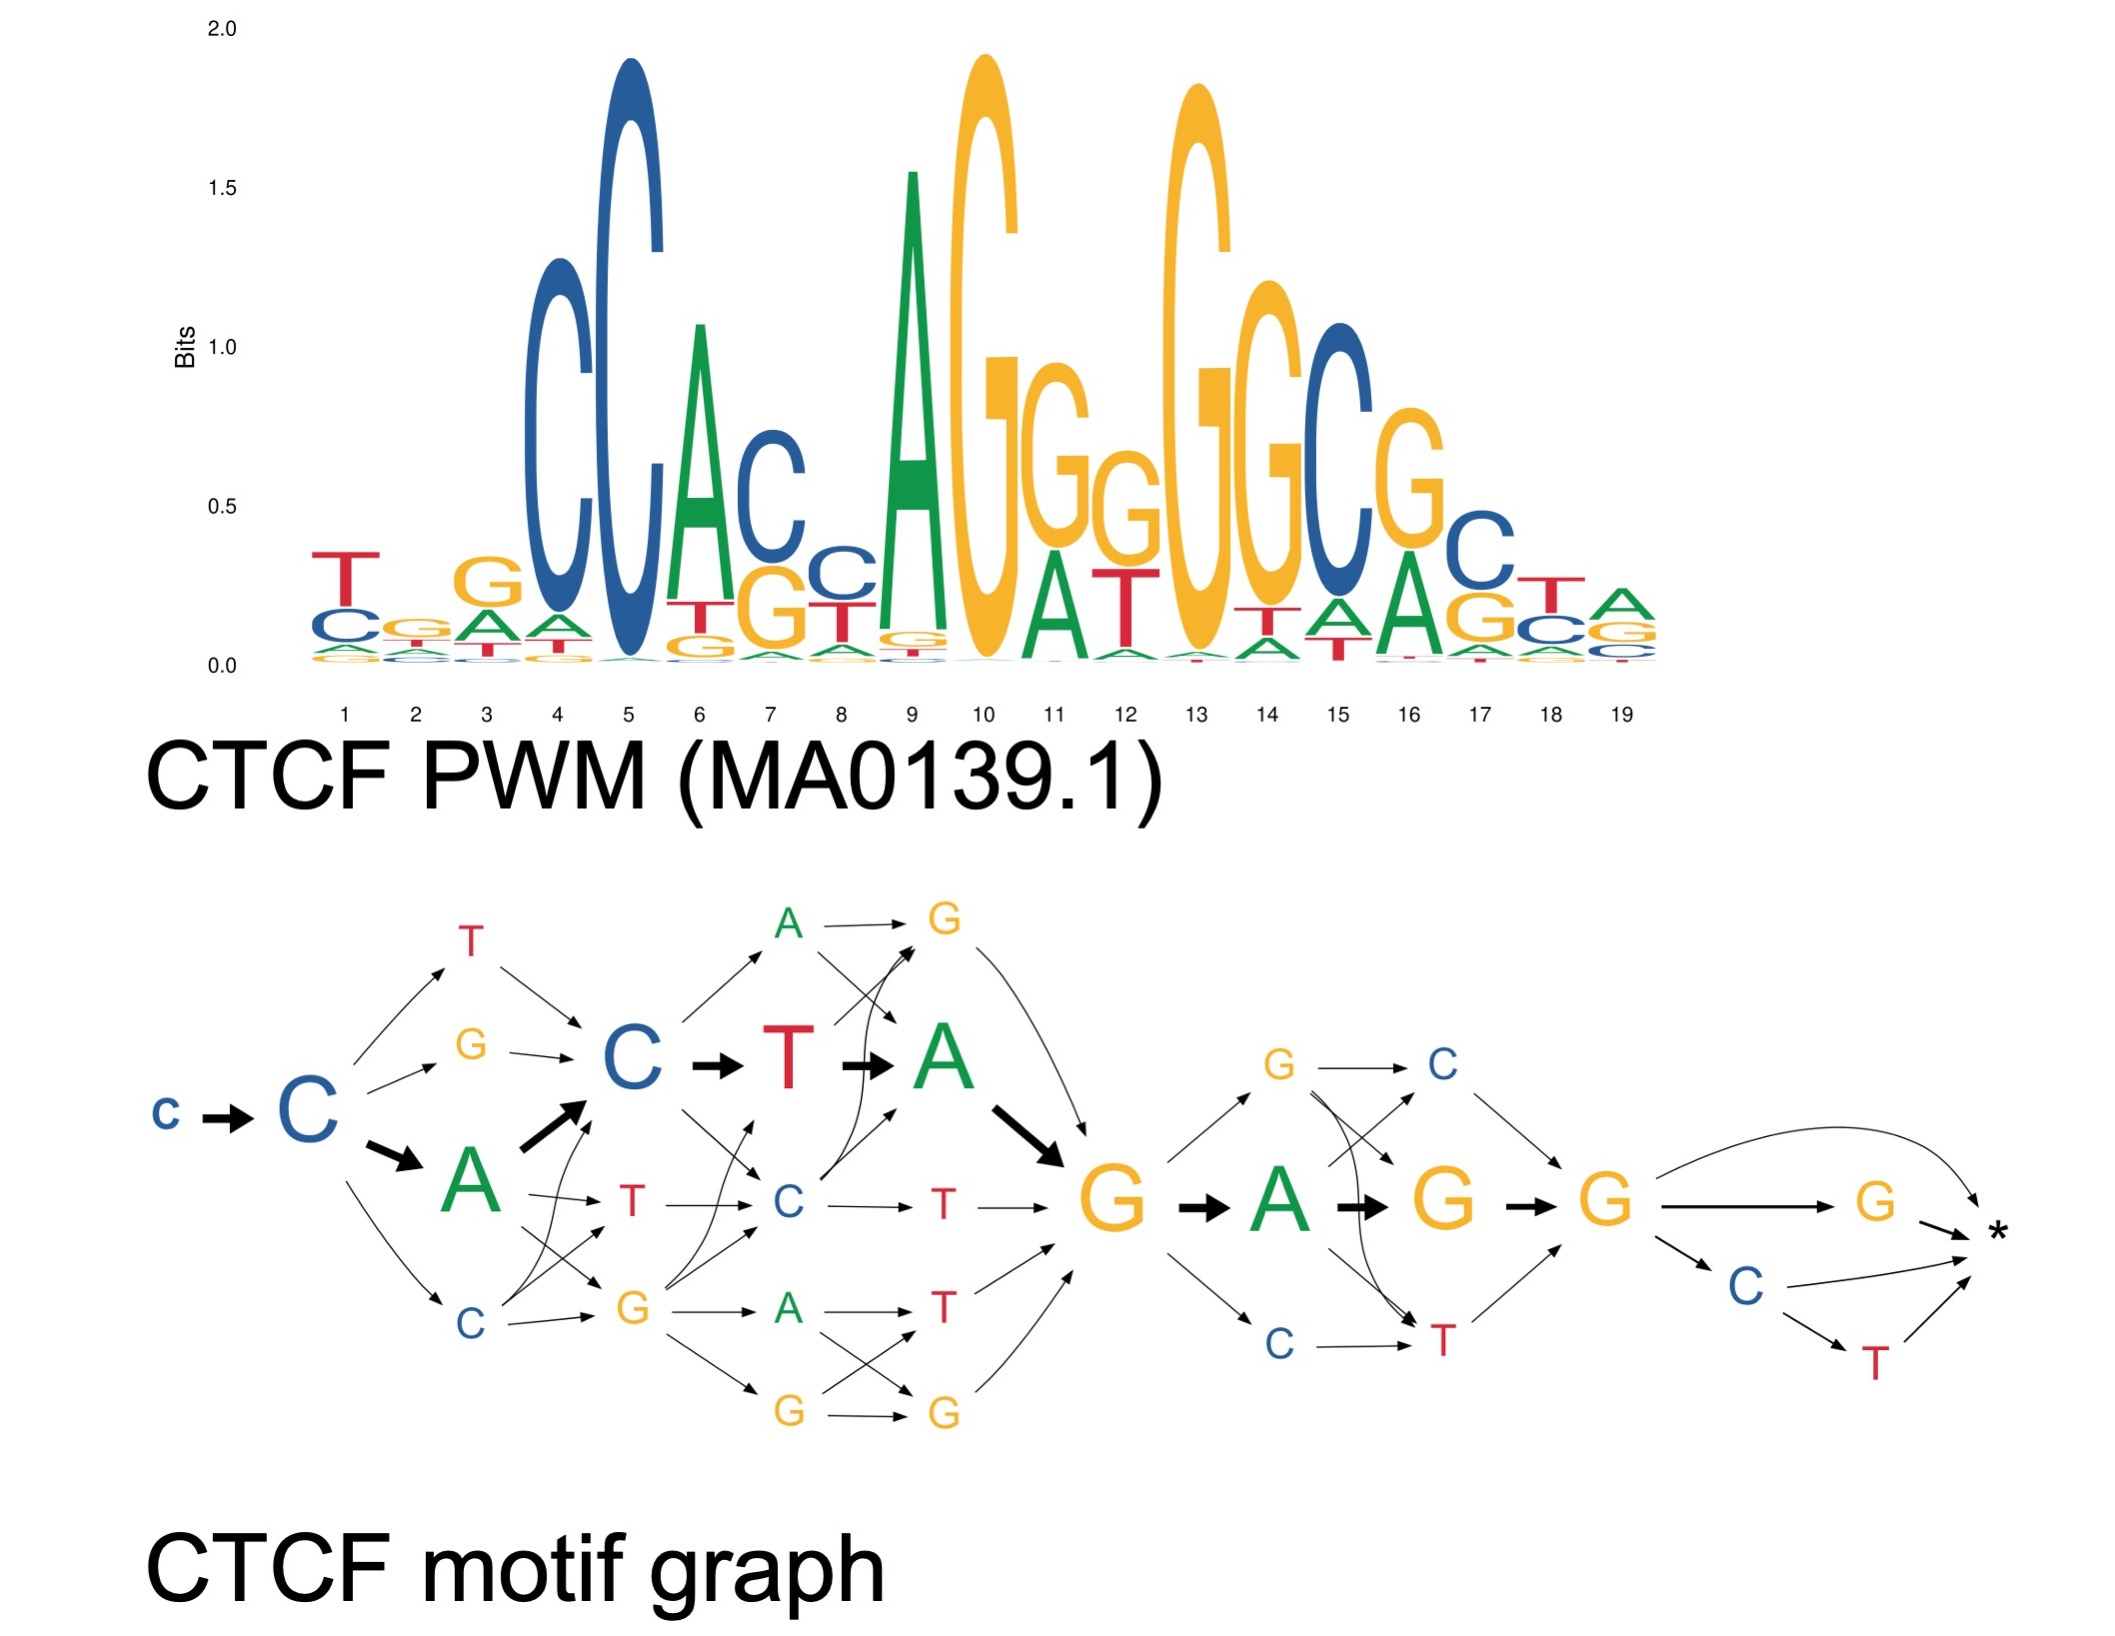
\includegraphics[width=\textwidth]{figures/ctcf_mg.jpg}
	\caption[Comparison between CTCF Motif Graph model and its PWM from the JASPAR database.]{\textbf{Comparison between CTCF MotifGraph model and its PWM from the JASPAR database.} On top the CTCF motif available on JASPAR database (MA0139.1). On the bottom the Motif Graph model trained using 100 $k$-mers obtained from a ChIP-seq experiment trageting CTCF binding site on HepG2 cell line.}
	\label{fig:ctcf_mg}
\end{figure} 
Moreover, such models would better predict the consequences of noncoding variants on TF-DNA binding events, and they could encode variable orders of nucleotide dependencies. Importantly, graph data structures are often interpretable and intuitive. With this aims in mind we developed the Motif Graph, a framework integrating the advantages of \emph{probabilistic graphical models-based} and \emph{SVM-based} motif discovery algorithms, without sacrificing model interpretability. A Motif Graph model $G$ is defined by a set of vertices $V$, a set of edges $E$, and a set of paths $P$. Each vertex $v \in V$ on the graph is labeled with a nucleotide, or mathematically $label(v) \in \{A, C, G, T\}$. Each edge $e \in E$ represents the allowed links between consecutive nucleotides in the TFBS motif. Each path $p \in P$ represents a \emph{haplotype} embedded in $G$, which correspond to one sequence used to train the Motif Graph model. Currently, the model is limited to encode $1$st order dependencies between consecutive nucleotides. However, the model is flexible and accomodate variable length motifs, beside recording the training sequences.
% ---- Motif Graph model construction
\section{Motif Graph model construction}
Motif Graph motif discovery procedure (\textbf{Algorithm \ref{algo:md_mg}}) is constitued of two main steps: $k$-mers prioritization, and graph model training and construction. To prioritize the $k$-mers Motif Graph currently employs the $k$-mer based motif discovery procedure implemented in Gkm-SVM \citep{ghandi2014enhanced}. Therefore, given a positive sequence dataset $S$ and a background dataset $B$, for each $k$-mer of length $k$ in $S$, the algorithm counts the number of matches in $S$ and in $B$, allowing mismatching positions (see \textbf{Section 2.1.2} for further details). Then, a similarity kernel is trained using the recovered $k$-mers frequencies. The trained kernel assigns to each $k$-mer in $S$ and in $B$ a weight proportional to its contribution in defining the foreground or the background dataset. The algorithm then ranks the $k$-mers according to their weight scores. The Motif Graph model is iteratively trained employing a greedy approach, which adds the top ranked $k$-mers to $G$ incrementally, one by one (see \textbf{Algorithm \ref{algo:mt_mg}} for details). Each $k$-mer is aligned to the current $G$ to maximize the number of nucleotides matching the current model. While aligning the $k$-mers to the current Motif Graph model, the algorithm shifts the input $k$-mer on the right and on the left up to a defined offset number of nucleotides. In our experiments with set the offset to $3$. Once built the model, we construct a scoring matrix similar to the widely used $PSSM$. However, our scoring matrix account for $1$st order dependencies between nucleotides, recalling the well-known DWMs (see \textbf{Section 2.1.3} for details). The scoring matrix is used to assign a likelihood score and classify new sequences as potentially bound or not bound by the investigated factor. In other words, the score describes how likely is the scanned sequence to contain a potential binding site. To score a sequence we slide the scoring matrix along the string employing a procedure similar to classical PWM scanning tools like FIMO \citep{grant2011fimo}.
\begin{algorithm}
	\DontPrintSemicolon
	\KwInput{$S$, $B$, $k$}
	\KwOutput{$G$}

	frequencies $\gets$ countFrequencies($S$, $B$, $k$)

	kernel $\gets$ trainKernel(frequencies)

	kmers, weights $\gets$ extractWeights(kernel)

	rankedKmer $\gets$ sort(kmers, weights)

	$G \gets \emptyset$

	\For{kmer in rankedKmers}
	{
		$G \gets$ addKmers($G$, kmer)
	}

	\Return{$G$}
	\caption{\textbf{Motif Graph motif discovery.}}
	\label{algo:md_mg}
\end{algorithm}
\begin{algorithm}
	\DontPrintSemicolon
	\KwInput{$G$, kmer, $i$}
	\KwOutput{$G$}
	
	\If{$i = 1$}
	{
		\Return{$G$}
	}

	\For{$j$ in $1$ to $3$}
	{
		matchesLeftOffset, alignmnetLeft $\gets$ countMatchesLeftOffset($G$, kmer, $j$)
	}

	\For{$j$ in $1$ to $3$}
	{
		matchesRightOffset, alignmnetRight $\gets$ countMatchesRightOffset($G$, kmer, $j$)
	}	
	
	alignment $\gets$ getBestAlignment(matchesLeftOffset, alignmentLeft, matchesRightOffset, alignmentRight)

	$G \gets$ insertKmer($G$, alignment)

	\Return{$G$}
	\caption{\textbf{Motif Graph model training.}}
	\label{algo:mt_mg}
\end{algorithm}
\section{Results}
To test our motif discovery algorithm we obtained $10,000$ ChIP-seq peak sequences from the ENCODE Project database \citep{encode2012integrated} for CTCF and GATA1 Transcription Factors, obtained on the HepG2 and K562 cell lines, respectively. The original ChIP-seq datasets were sorted according to the peaks enrichment score in decreasing order, in order to test our algorithm on reliable peaks. Interestingly, the trained Motif Graph models were closed to the motifs PWM available on the JASPAR database \citep{sandelin2004jaspar} for both CTCF and GATA1 (\textbf{Fig.\ref{fig:ctcf_mg}} and \textbf{Fig.\ref{fig:gata1_mg}}). For both TFs, the Motif Graph models captured the main motif sequence. The main motifs are also enforced by the edge thickness which is proportional to the number of training $k$-mers supporting each $p \in P$.
\begin{figure}
	\centering
	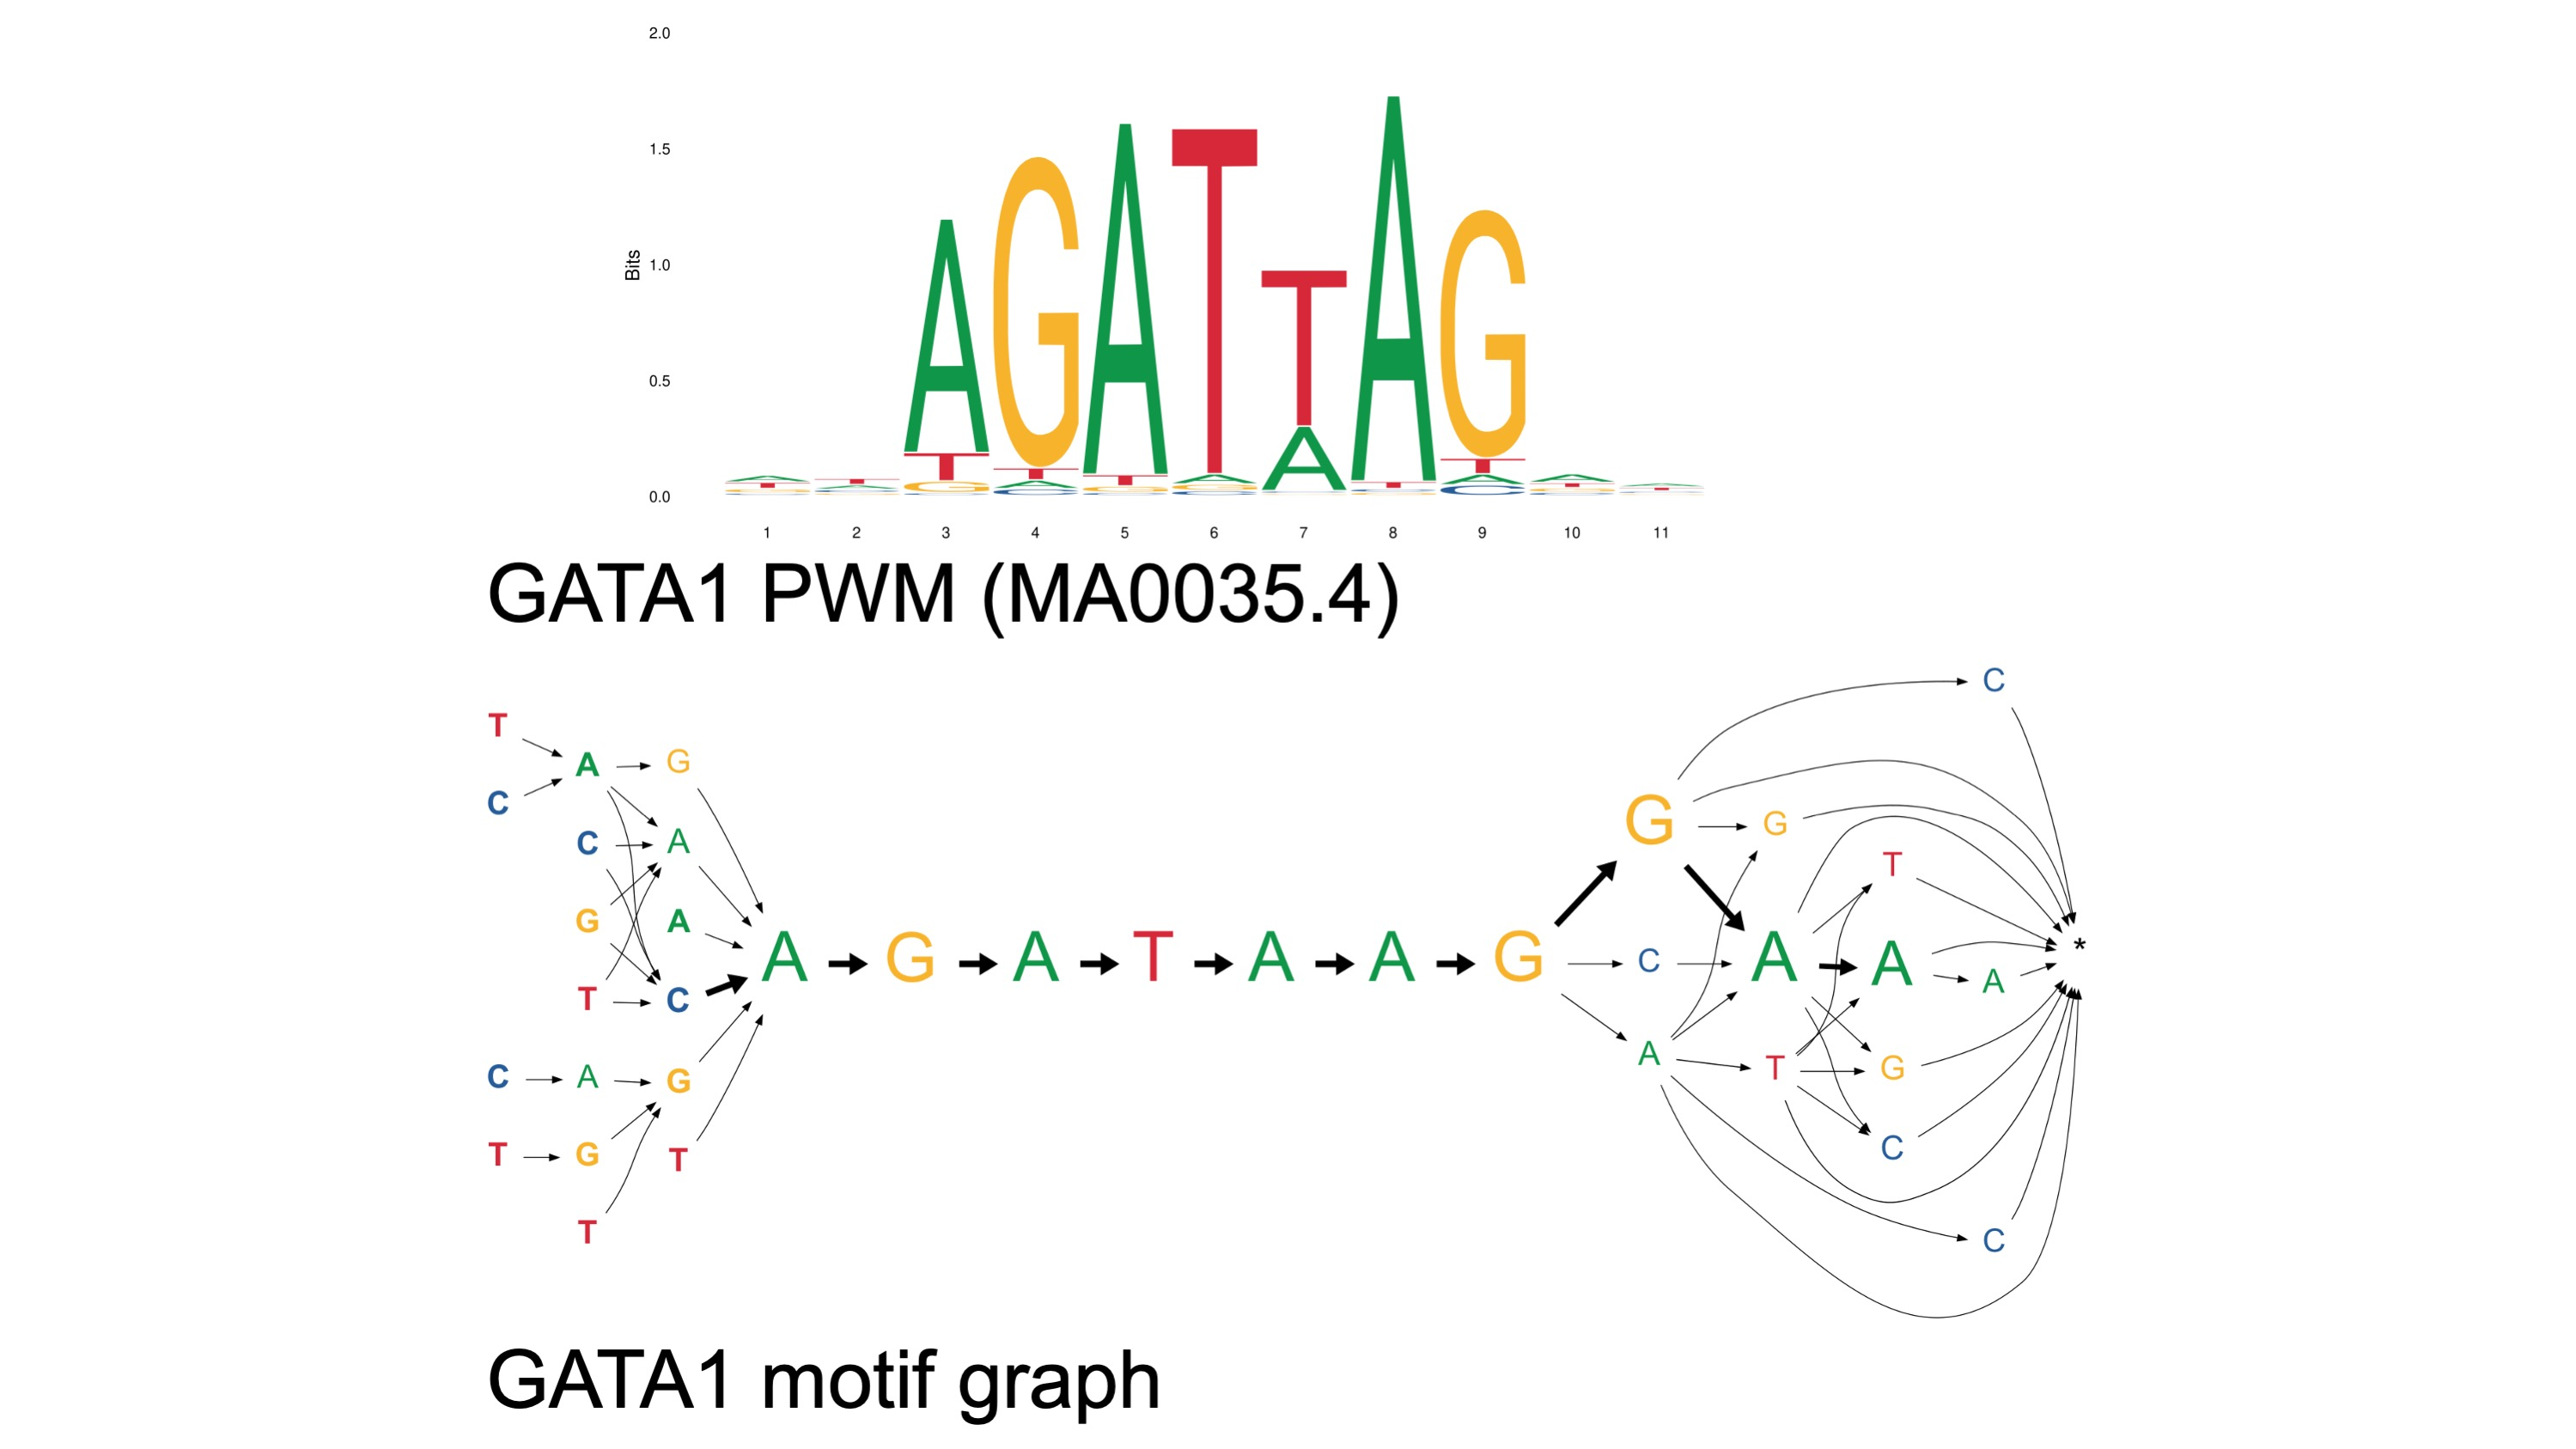
\includegraphics[width=\textwidth]{figures/gata1_mg.jpg}
	\caption[Comparison between GATA1 Motif Graph model and its PWM from the JASPAR database.]{\textbf{Comparison between GATA1 MotifGraph model and its PWM from the JASPAR database.} On top the GATA1 motif available on JASPAR database (MA0035.4). On the bottom the Motif Graph model trained using 100 $k$-mers obtained from a ChIP-seq experiment trageting GATA1 binding site on K562 cell line.}
	\label{fig:gata1_mg}
\end{figure} 
Then, we tested the discriminative performance of both Motif Graph model, with different number of training $k$-mers (\textbf{Fig.\ref{fig:dp_mg}}), to establish the optimal number of training sequences for the CTCF and GATA1 Motif Graph models. To compare the models discriminative performance, we performed a cross-validation experiment using splitting the $S$ and $B$ dataset in training and testing set (75\% and 25\%, respectively). We trained the models with $10$, $50$, $100$, $200$, $350$, $500$, and $750$ $k$-mers. For CTCF the best prformance in terms of both AUC ($0.72$) and F1-score ($0.71$) were obtained training the Motif Graph on $100$ $k$-mers (\textbf{Table \ref{table:ctcf_auc_f1}}). For GATA1 the model returned the best AUC using $200$ $k$-mers ($0.76$), while the best F1-score ($0.70$) was obtained training the model with $100$ sequences (\textbf{Table \ref{table:gata1_auc_f1}}).
\begin{figure}
	\centering
	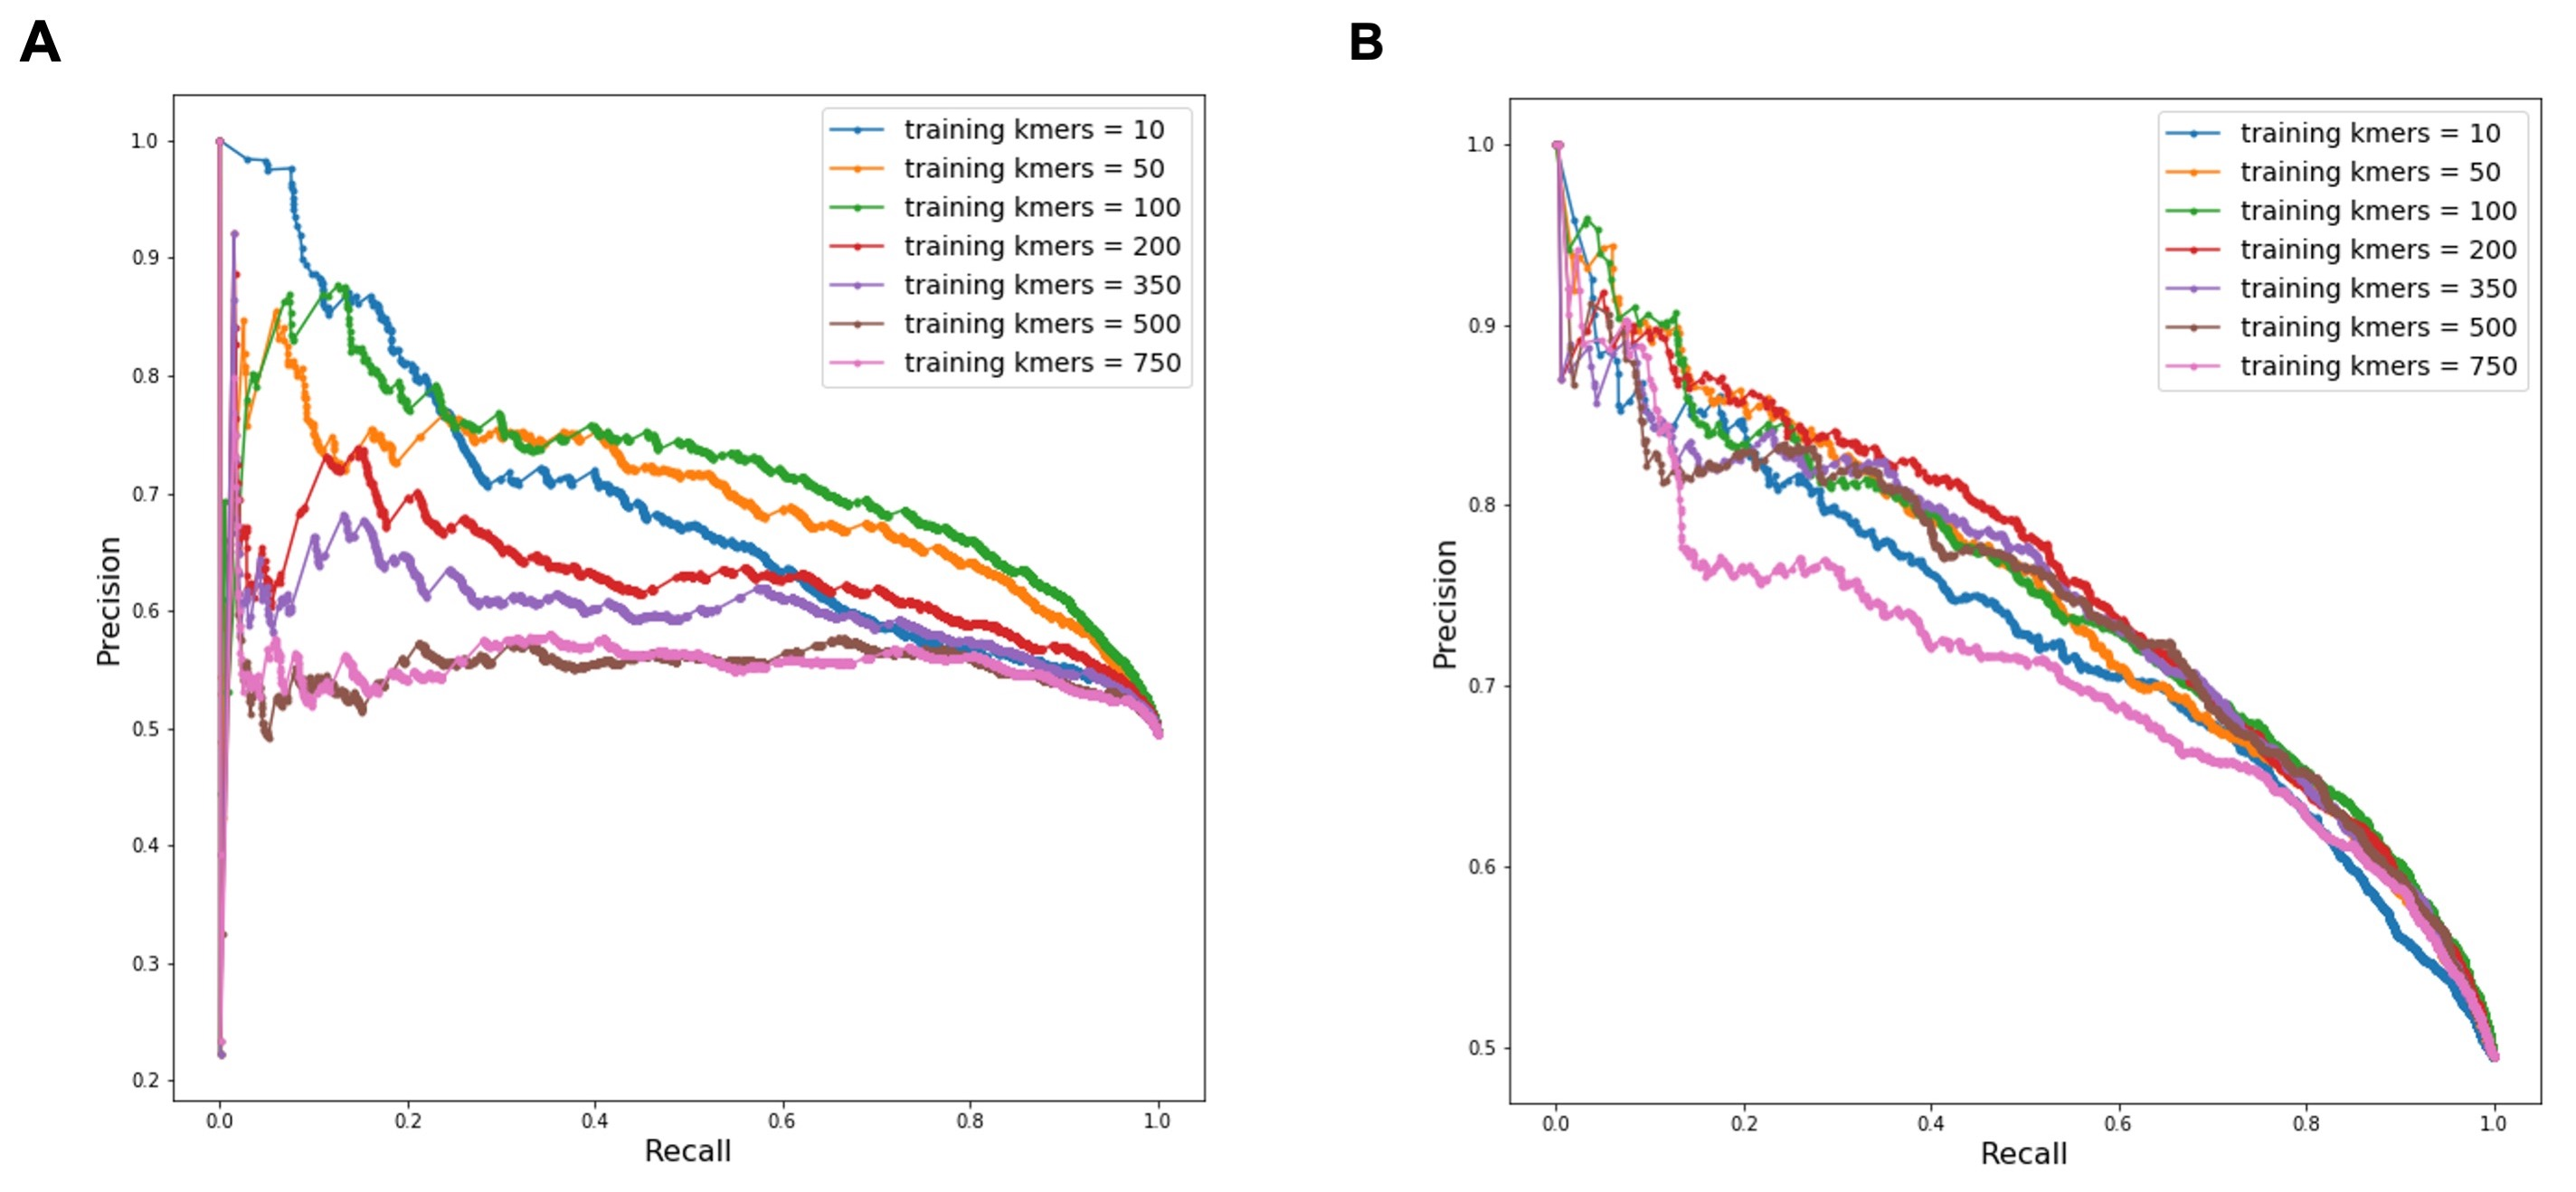
\includegraphics[width=\textwidth]{figures/dp_mg.jpg}
	\caption[Precision-Recall curves obtained varying the number of $k$-mers used to train the Motif Graph models.]{\textbf{Precision-Recall curves obtained varying the number of $k$-mers used to train the Motif Graph models.} To establish the number of training $k$-mers returning the best discriminative performance we computed the Precision-Recall curves of different Motif Graph models trained using 10, 50, 100, 200, 350, 500, and 750 $k$-mers on \textbf{(A)} CTCF and \textbf{(B)} GATA1}
	\label{fig:dp_mg}
\end{figure} 
\begin{table}
	\centering
	\begin{tabular}{|p{3cm}|p{1.cm}|p{1.cm}|p{1.cm}|p{1.cm}|p{1.cm}|p{1.cm}|p{1.cm}|}
		\hline
		\textbf{Training $k$-mers}& \textbf{$10$}& \textbf{$50$}& \textbf{$100$}& \textbf{$200$}& \textbf{$350$}& \textbf{$500$}& \textbf{$750$} \\
		\hline
		\textbf{AUC}& $0.69$& $0.69$& $0.72$& $0.63$& $0.60$& $0.55$& $0.55$\\
		\hline
		\textbf{F1-score}& $0.62$& $0.69$& $0.71$& $0.65$& $0.62$& $0.57$& $0.56$\\
		\hline
	\end{tabular}
	\caption[CTCF Motif Graph model AUC and F1-scores values with different number of training $k$-mers.]{\textbf{CTCF Motif Graph model AUC and F1-scores values with different number of training $k$-mers.}}
	\label{table:ctcf_auc_f1}
\end{table}
\begin{table}
	\centering
	\begin{tabular}{|p{3cm}|p{1.cm}|p{1.cm}|p{1.cm}|p{1.cm}|p{1.cm}|p{1.cm}|p{1.cm}|}
		\hline
		\textbf{Training $k$-mers}& \textbf{$10$}& \textbf{$50$}& \textbf{$100$}& \textbf{$200$}& \textbf{$350$}& \textbf{$500$}& \textbf{$750$} \\
		\hline
		\textbf{AUC}& $0.73$& $0.75$& $0.75$& $0.76$& $0.74$& $0.74$& $0.71$\\
		\hline
		\textbf{F1-score}& $0.68$& $0.68$& $0.70$& $0.69$& $0.70$& $0.69$& $0.67$\\
		\hline
	\end{tabular}
	\caption[GATA1 Motif Graph model AUC and F1-scores values with different number of training $k$-mers.]{\textbf{GATA1 Motif Graph model AUC and F1-scores values with different number of training $k$-mers.}}
	\label{table:gata1_auc_f1}
\end{table}
Then, we compared the Motif Graph models discriminative performance against the corresponding PWM and DWM models, recovered from JASPAR \citep{sandelin2004jaspar} and HOCOMOCO \citep{kulakovskiy2016hocomoco} databases, respectively. For CTCF, both the PWM and the DWM models returned better predictive performance than our model (\textbf{Fig.\ref{fig:dp_mg_pwm_dwm} (A)}). On the other hand, on GATA1 data our model showed better performance than PWMs, but still performed worse than DWMs (\textbf{Fig.\ref{fig:dp_mg_pwm_dwm} (B)}).
\begin{figure}
	\centering
	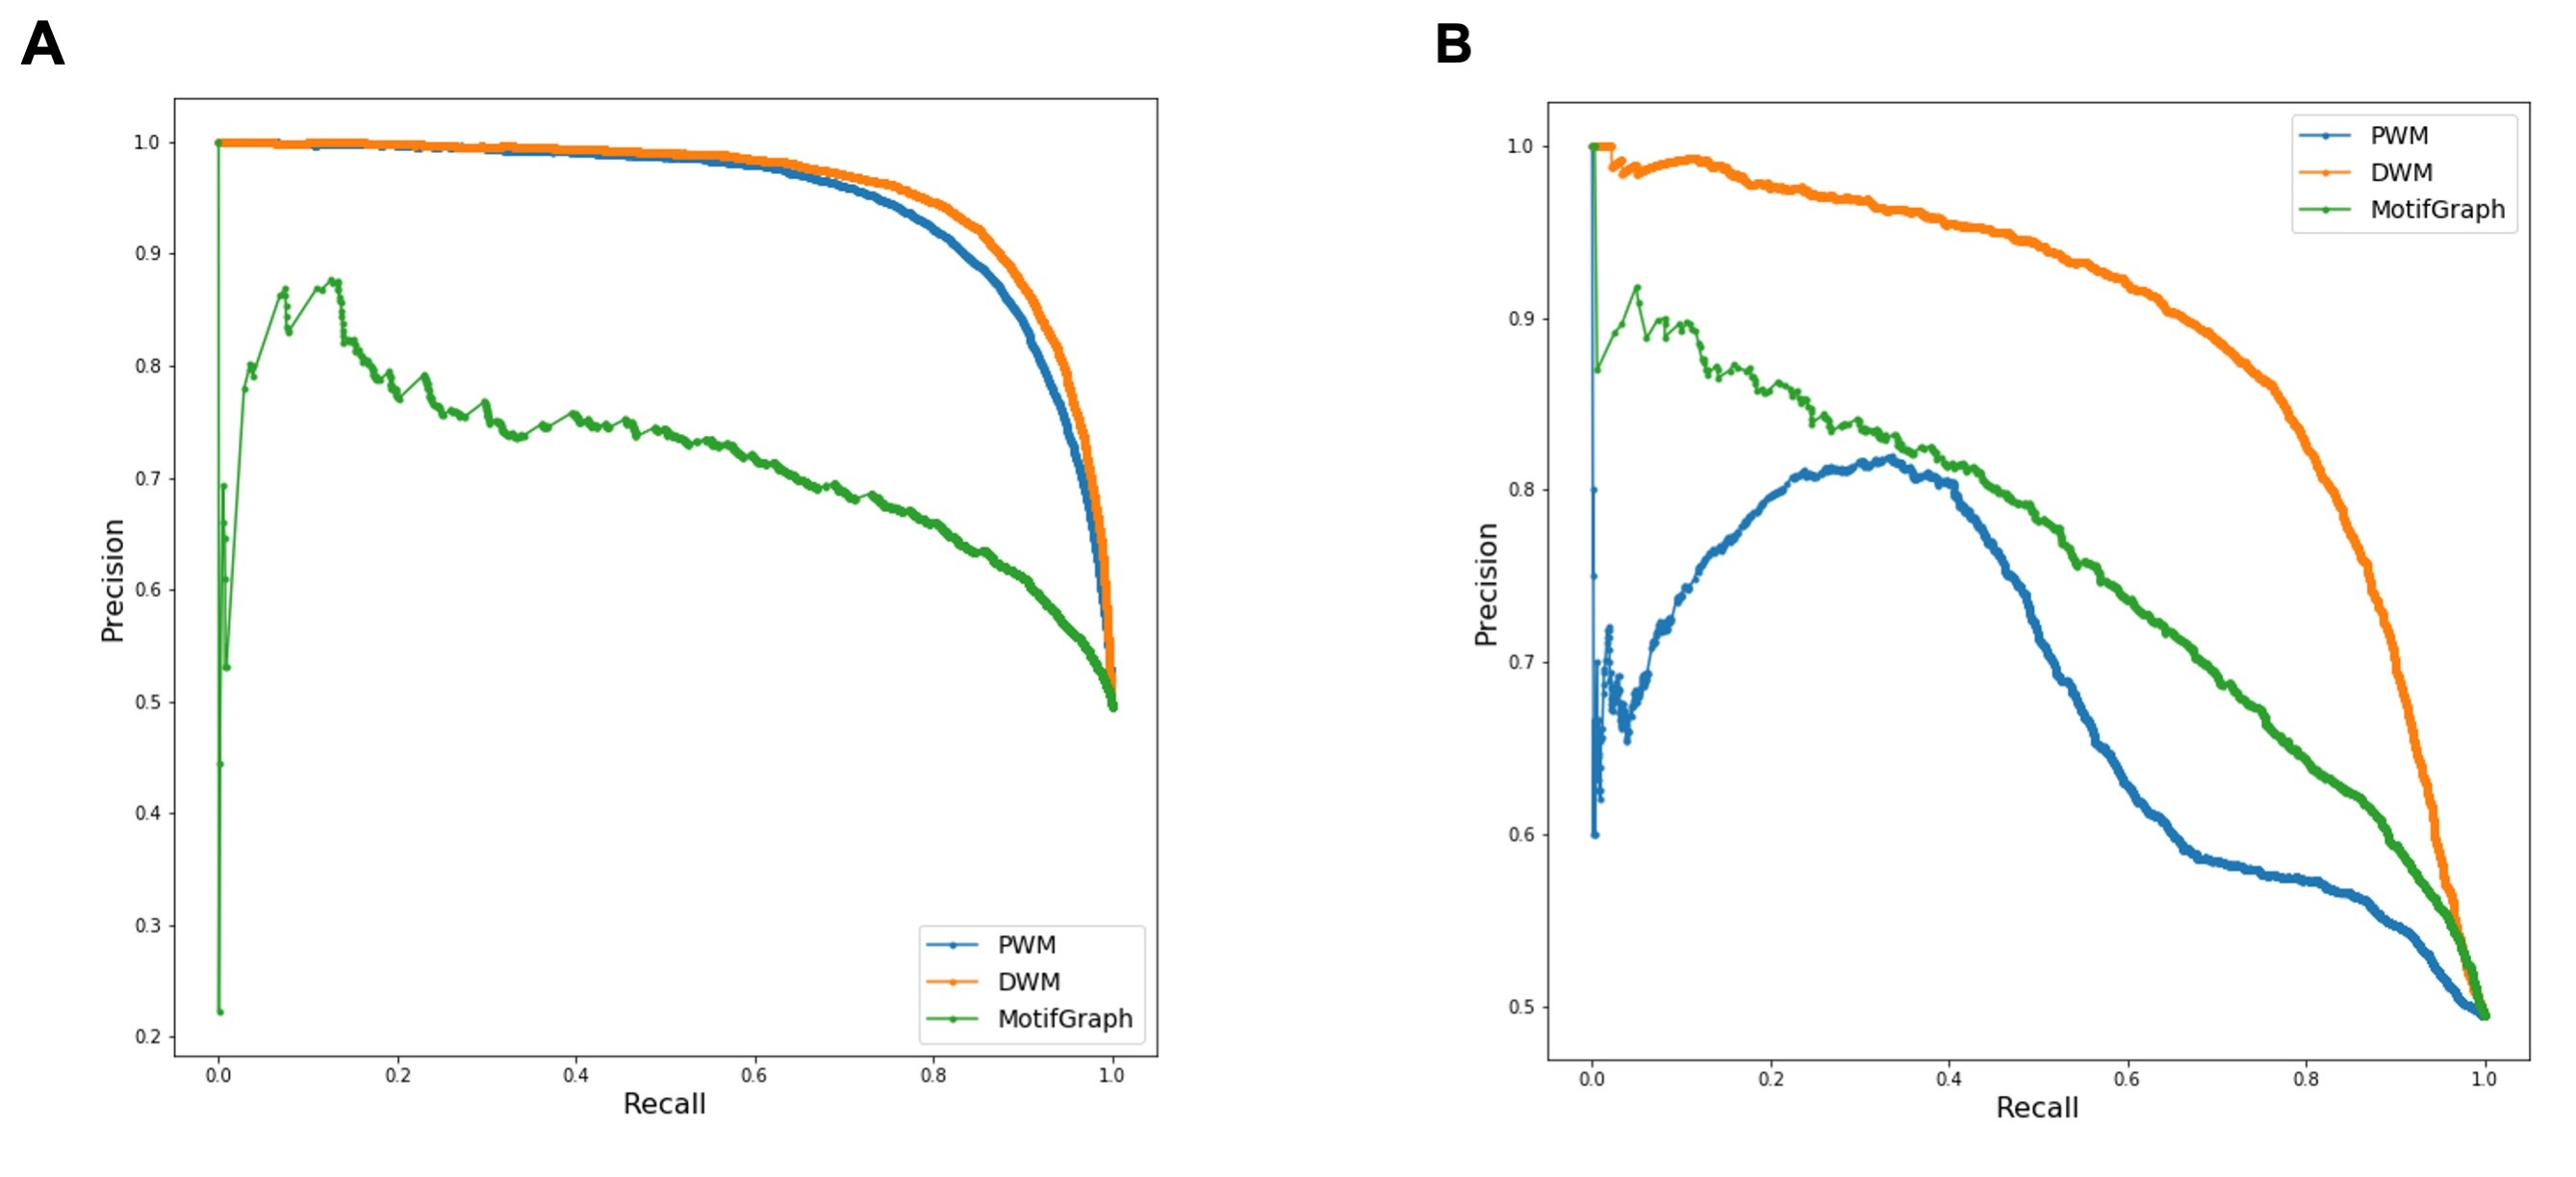
\includegraphics[width=\textwidth]{figures/dp_mg_pwm_dwm.jpg}
	\caption[Comparing Motif Graph, PWM, and DWM Precision-Recall curves.]{\textbf{Comparing Motif Graph, PWM, and DWM Precision-Recall curves.} We compared the discriminative power of the Motif Graph models against that of PWMs and DWMs for both \textbf{(A)} CTCF and \textbf{(B)} GATA1.}
	\label{fig:dp_mg_pwm_dwm}
\end{figure} 


% ------  begin bibliography
\bibliography{biblio}
\bibliographystyle{natbib}





\end{document}